\documentclass[a4paper,11pt]{article}

\usepackage[T1]{fontenc}
\usepackage[indonesian]{babel}
\usepackage{lmodern}
\usepackage[top=0.8in,bottom=1in,left=1in,right=1in]{geometry}
\usepackage{graphicx}
\usepackage{amsmath}
\usepackage{booktabs,tabularx}
\usepackage{listings}
\usepackage{fancyhdr,lastpage}
\usepackage[normalem]{ulem}
\usepackage[unicode,hidelinks]{hyperref}

\newcommand{\namakelompok}{G06 PhilippsLeatherJacket}
\setcounter{tocdepth}{2}
\lstset{language=Python,basicstyle=\ttfamily\footnotesize,breaklines=true}

\pagestyle{fancy}
\fancyhf{}
\setlength{\headheight}{34pt}
\setlength{\headsep}{18pt}
\fancyhead[L]{%
  
\includegraphics[height=20pt]{assets/logos/itb.pdf}\hspace{0.8em}%
  
\includegraphics[height=20pt]{assets/logos/stei.pdf}%
}
\fancyhead[R]{\footnotesize
  \shortstack[r]{\textbf{IF3170 Inteligensi Artifisial}\\
    Laporan Tugas Besar 2\\
    \textit{Semester I 2026/2027}}%
}
\renewcommand{\footrulewidth}{0.4pt}
\fancyfoot[L]{\footnotesize\namakelompok}
\fancyfoot[R]{\footnotesize Halaman \thepage{} dari \pageref*{LastPage}}

\hypersetup{
  pdftitle={Laporan Tugas Besar 2 IF3170},
  pdfauthor={G06 PhilippsLeatherJacket},
  bookmarksnumbered=true,
  linktoc=all
}


\begin{document}
\hypersetup{pageanchor=false}
\begin{titlepage}
  \centering
  \vspace*{10mm}
  {\LARGE\bfseries Laporan Tugas Besar 2\par}
  \vspace{3mm}
  {\Large\scshape IF3170 Inteligensi Artifisial\par}
  \vspace{2mm}
  {\normalsize Semester I Tahun 2026/2027\par}

  \vfill
  
\includegraphics[width=43mm]{assets/logos/itb.pdf}
  \vfill

  {\large\scshape Kelompok \namakelompok\par}
  \vspace{6mm}
  \begin{tabular}{@{}lr@{}}
    Stevanus Agustaf Wongso & 13524020 \\
    Jonathan Kris Wicaksono & 13524023 \\
    Made Branenda Jordhy & 13524026 \\
    Ray Owen Martin & 13524033 \\
    Philipp Hamara & 13524101 \\
  \end{tabular}

  \vfill
  {\large\scshape Program Studi Teknik Informatika\par}
  Sekolah Teknik Elektro dan Informatika\par
  Institut Teknologi Bandung\par
  \vspace*{9mm}
\end{titlepage}
\hypersetup{pageanchor=true}

\tableofcontents
\clearpage

\section{Deskripsi Persoalan}

\subsection{Konteks dan Tujuan}

\subsection{Dataset dan Variabel Target}

\subsection{Eksplorasi Data}

\section{Pembahasan}

\subsection{Cleaning dan Preprocessing}
\label{subsec:preprocessing}

Tahap prapemrosesan data (\textit{data preprocessing}) dan pembersihan (\textit{data cleaning})
merupakan fondasi kritis sebelum data disalurkan ke model klasifikasi. Kualitas data mentah
sangat menentukan kemampuan generalisasi model pembelajaran mesin. Seluruh rangkaian prapemrosesan
diimplementasikan secara modular pada paket \texttt{src/preprocess/} dan dieksekusi secara
terintegrasi melalui fungsi \texttt{run\_preprocessing}. Alur ini terdiri atas tiga tahapan utama:
pembersihan data, transformasi data, serta seleksi fitur dan reduksi dimensi.

\subsubsection{Pembersihan Data}

Tahap pembersihan data menangani tiga anomali utama pada dataset mentah:

\paragraph{Penanganan Nilai Hilang (\textit{Missing Values}).}
Pemeriksaan pada dataset latih dan uji menunjukkan adanya nilai kosong (\textit{missing values})
pada sejumlah atribut numerik dan kategorikal. Nilai yang hilang diimputasi menggunakan statistik
yang dipelajari semata-mata dari data latih guna mencegah kebocoran data (\textit{data leakage}):
\begin{itemize}
  \item \textbf{Fitur Numerik}: Diimputasi menggunakan nilai median data latih:
        \[
        x_{\text{impute}} = \text{median}(X_{\text{train}, j}) .
        \]
        Median dipilih daripada \textit{mean} karena median bersifat kekal (\textit{robust}) terhadap nilai-nilai
        ekstrem (\textit{outliers}) pada kolom seperti \texttt{nightly\_rate\_idr} dan \texttt{days\_before\_arrival}.
        Untuk atribut diskrit seperti \texttt{num\_children}, nilai kosong diisi dengan modus atau 0.
  \item \textbf{Fitur Kategorikal}: Diimputasi menggunakan nilai modus (\textit{most frequent value})
        dari data latih agar konsisten dengan kategori dominan.
\end{itemize}

\paragraph{Penanganan Data Ganda (\textit{Duplicates}).}
Deteksi duplikasi baris identik dilakukan menggunakan fungsi \texttt{df.duplicated()}. Baris-baris
yang memiliki nilai sama persis di seluruh kolom diidentifikasi dan ditangani untuk mencegah pembobotan
berlebih (\textit{over-representation}) dari instans yang identik pada fungsi objektif model.

\paragraph{Penanganan Data Tidak Valid (\textit{Invalid Data}).}
Berdasarkan pemahaman domain reservasi perhotelan, didefinisikan kriteria data yang tidak valid secara logis:
\begin{enumerate}
  \item Nilai numerik bernilai negatif ($< 0$), yang tidak masuk akal untuk kuantitas orang, malam, atau biaya.
  \item Reservasi tanpa tamu dewasa (\texttt{num\_adults == 0}), karena reservasi hotel memerlukan penanggung jawab dewasa.
  \item Reservasi dengan total durasi menginap 0 malam (\texttt{weekend\_nights + weekday\_nights == 0}).
  \item Tanggal kedatangan yang tidak valid secara kalender (misalnya tanggal 29 Februari pada tahun non-kabisat).
\end{enumerate}
Strategi penanganannya dibedakan secara tegas antara data latih dan data uji:
\begin{itemize}
  \item \textbf{Data Latih}: Baris-baris tidak valid dihapus (\textit{dropped}) karena jumlahnya relatif kecil
        ($< 200$ baris) sehingga tidak mengurangi ukuran data latih secara signifikan, namun efektif menjaga
        kebersihan distribusi data latih.
  \item \textbf{Data Uji}: Baris tidak valid \textbf{tidak boleh dihapus} agar jumlah baris submisi tetap utuh
        (6.844 baris). Nilai yang tidak valid pada data uji diperbaiki (\textit{repaired}) dengan menggantikannya
        menggunakan nilai median yang dipelajari dari data latih.
\end{itemize}

\subsubsection{Transformasi Data}

\paragraph{Pengodean Fitur Kategorikal (\textit{Categorical Encoding}).}
Model pembelajaran mesin berbasis aljabar linier dan geometri memerlukan representasi numerik.
Dua pendekatan pengodean diterapkan berdasarkan sifat skala variabelnya:
\begin{itemize}
  \item \textbf{\textit{Ordinal Encoding}}: Diterapkan pada fitur bertingkat (ordinal) yang memiliki urutan logis,
        khususnya \texttt{meal\_package}:
        \[
        \text{"Room Only"} \mapsto 1,\quad \text{"Breakfast"} \mapsto 2,\quad \text{"Half Board"} \mapsto 3,\quad \text{"Full Board"} \mapsto 4 .
        \]
        Pemetaan ini mempertahankan informasi urutan dan tingkat kelengkapan paket makan tanpa menambah dimensi fitur.
  \item \textbf{\textit{One-Hot Encoding}}: Diterapkan pada fitur nominal tanpa hierarki urutan, yaitu \texttt{room\_category}
        dan \texttt{booking\_channel}. Digunakan parameter \texttt{drop\_first=True} untuk membuang satu kategori basis
        guna mencegah multikolinearitas sempurna (\textit{dummy variable trap}). Kolom pada data uji secara eksplisit
        diselaraskan (\textit{reindexed}) dengan data latih agar dimensi kedua himpunan data selalu konsisten.
\end{itemize}

\paragraph{Penskalaan Fitur (\textit{Feature Scaling}).}
Atribut numerik memiliki rentang skala yang sangat beragam, mulai dari jumlah orang ($1$--$4$) hingga harga per malam
\texttt{nightly\_rate\_idr} yang mencapai ratusan ribu hingga jutaan rupiah. Variabel dengan rentang besar akan
mendominasi fungsi jarak atau gradien secara tidak proporsional. Oleh karena itu, seluruh fitur numerik distandarisasi
menggunakan \texttt{StandardScaler}:
\[
z = \frac{x - \mu}{\sigma} ,
\]
di mana $\mu$ adalah rerata dan $\sigma$ adalah standar deviasi yang dihitung semata-mata dari data latih.
Penskalaan ini krusial untuk algoritma berbasis jarak seperti KNN dan berbasis margin seperti SVM.

\paragraph{Penanganan Ketidakseimbangan Kelas (\textit{Class Imbalance}).}
Dataset pembatalan hotel memiliki distribusi target \texttt{is\_canceled} yang tidak seimbang, dengan kelas
positif (dibatalkan) mencakup sekitar $32{,}77\%$ dan kelas negatif (tidak batal) sebesar $67{,}23\%$.
Untuk model yang rentan bias terhadap kelas mayoritas, diterapkan teknik \textit{oversampling} sintetis
\textbf{SMOTE} (\textit{Synthetic Minority Over-sampling Technique}). SMOTE bekerja dengan cara membangkitkan
sampel sintetis baru pada segmen garis yang menghubungkan titik kelas minoritas dengan $k$ tetangga terdekatnya:
\[
x_{\text{baru}} = x_i + \lambda (x_{zi} - x_i), \quad \lambda \sim \mathcal{U}(0, 1) .
\]
Penerapan SMOTE dibatasi secara ketat hanya pada data latih, dan tidak pernah diterapkan pada himpunan validasi
maupun data uji guna menjamin keaslian evaluasi performa model.

\subsubsection{Seleksi Fitur dan Reduksi Dimensi}

\paragraph{Seleksi Fitur Univariat (\textit{SelectKBest}).}
Untuk membuang fitur-fitur yang tidak informatif atau memiliki korelasi rendah terhadap target, digunakan
metode seleksi univariat \texttt{SelectKBest} dengan uji statistik ANOVA F-Value (\texttt{f\_classif}):
\[
F = \frac{\text{MSB}}{\text{MSW}} = \frac{\sum_{c} n_c (\bar{x}_c - \bar{x})^2 / (K - 1)}{\sum_{c} \sum_{i} (x_{ci} - \bar{x}_c)^2 / (N - K)} ,
\]
di mana $\text{MSB}$ mengukur varians antarkelompok kelas dan $\text{MSW}$ mengukur varians di dalam kelompok kelas.
Dipilih $K = 15$ fitur teratas dengan skor tertinggi. Hasil pemeringkatan menunjukkan bahwa fitur-fitur seperti
\texttt{days\_before\_arrival}, \texttt{special\_requests}, \texttt{arrival\_year}, dan \texttt{nightly\_rate\_idr}
memiliki kontribusi diskriminasi paling dominan dalam membedakan reservasi yang dibatalkan dan yang tidak.

\paragraph{Reduksi Dimensi Principal Component Analysis (PCA).}
Setelah seleksi 15 fitur terbaik, diterapkan teknik \textit{Principal Component Analysis} (PCA) untuk
mengatasi fenomena \textit{Curse of Dimensionality} (kutukan dimensi) dan mereduksi redundansi antarkomponen.
PCA mencari arah vektor eigen yang memaksimalkan variansi proyeksi data melalui dekomposisi matriks kovarians:
\[
\mathbf{\Sigma} v_i = \lambda_i v_i .
\]
Dengan menentukan batas retensi variansi kumulatif sebesar $95\%$ ($\sum_{i=1}^m \lambda_i / \sum_{j=1}^d \lambda_j \ge 0{,}95$),
dimensi data berhasil direduksi secara signifikan dari 15 fitur menjadi \textbf{9 komponen utama}.
Reduksi ini mempertahankan informasi krusial data sekaligus meningkatkan efisiensi waktu komputasi jarak pada model KNN.

\subsection{Metodologi Validasi dan Metrik}

Untuk mengevaluasi performa kelima model klasifikasi secara objektif dan menghindari \textit{data leakage},
diterapkan metodologi pemisahan data yang ketat dan pemilihan metrik evaluasi yang representatif.

\paragraph{Skema Pembagian Data dan Validasi Silang.}
Data latih dibagi menjadi data latih dan data validasi dengan rasio $85:15$ menggunakan teknik
pembagian terstratifikasi (\textit{stratified train-validation split}). Stratifikasi dilakukan tidak hanya
berdasarkan label target $y \in \{0, 1\}$, melainkan juga terhadap indikator data asli versus sintetis SMOTE.
Selain itu, pengujian kestabilan hiperparameter menggunakan \textit{Stratified 5-Fold Cross Validation}.
Kaidah validasi paling mendasar yang diterapkan adalah: \textbf{seluruh metrik evaluasi hanya dihitung pada baris
data asli} (\textit{original rows only}), sedangkan sampel sintetis SMOTE tidak pernah diikutsertakan dalam kalkulasi
skor evaluasi. Hal ini menjamin bahwa metrik yang dilaporkan mencerminkan performa nyata terhadap distribusi data sebenarnya.

\paragraph{Metrik Evaluasi.}
Karena terdapat ketidakseimbangan kelas ($32{,}77\%$ kelas positif), akurasi standar dapat memberikan
ilusi performa tinggi padahal model mengabaikan kelas minoritas. Oleh sebab itu, rangkaian metrik berikut digunakan:
\begin{enumerate}
  \item \textbf{Akurasi}:
        \[
        \text{Akurasi} = \frac{TP + TN}{TP + TN + FP + FN}
        \]
  \item \textbf{Presisi dan \textit{Recall} per Kelas}:
        \[
        \text{Presisi}_c = \frac{TP_c}{TP_c + FP_c}, \qquad \text{Recall}_c = \frac{TP_c}{TP_c + FN_c}
        \]
  \item \textbf{Macro-Averaged F1-Score (Metrik Utama)}:
        \[
        \text{Macro-F1} = \frac{1}{|\mathcal{C}|} \sum_{c \in \mathcal{C}} \frac{2 \cdot \text{Presisi}_c \cdot \text{Recall}_c}{\text{Presisi}_c + \text{Recall}_c}
        \]
        \textit{Macro-F1} menghitung nilai rata-rata F1 unweighted antarkelas, sehingga kelas pembatalan ($1$)
        dan non-batal ($0$) memiliki bobot kepentingan yang setara terlepas dari jumlah frekuensinya.
  \item \textbf{Matriks Konfusi (\textit{Confusion Matrix})}:
        Memetakan perbandingan langsung antara label aktual dan label prediksi guna mendeteksi kecenderungan
        kesalahan tipe I (\textit{False Positive}) dan kesalahan tipe II (\textit{False Negative}).
\end{enumerate}

\subsection{\textit{k}-Nearest Neighbors (KNN)}

\textit{k}-Nearest Neighbors (KNN) merupakan algoritma pembelajaran mesin non-parametrik
berbasis instans (\textit{instance-based learning}) yang tergolong sebagai \textit{lazy learner}.
KNN tidak membentuk fungsi pemetaan eksplisit selama tahap pelatihan, melainkan menyimpan
seluruh sampel data latih dan menunda seluruh proses komputasi hingga tahap inferensi.
Untuk mengklasifikasikan sampel kueri $x \in \mathbf{R}^d$, KNN mengukur jarak antara $x$
dengan seluruh data latih, memilih $k$ tetangga terdekat $\mathcal{N}_k(x)$, lalu
menentukan kelas prediksi berdasarkan agregasi label dari tetangga-tetangga tersebut.

Jarak antara dua titik data $x, z \in \mathbf{R}^d$ dihitung menggunakan metrik jarak
Minkowski tingkat $p$:
\[
D(x, z) = \left( \sum_{j=1}^d |x_j - z_j|^p \right)^{\frac{1}{p}} .
\]
Kasus khusus dari metrik ini mencakup jarak Manhattan ($p=1$) dan jarak Euclidean ($p=2$).
Untuk fitur berskala biner atau kategorikal, jarak Hamming ternormalisasi didefinisikan sebagai
$D_{\text{Hamming}}(x, z) = \frac{1}{d} \sum_{j=1}^d [x_j \neq z_j]$, dengan $[P]$ bernilai 1 jika kondisi $P$ benar dan 0 jika sebaliknya (notasi Iverson).

Pada skema penentuan label mayoritas (\textit{majority voting}), prediksi kelas ditentukan
melalui pembobotan seragam (\textit{uniform}):
\[
\hat{y} = \arg\max_{c \in \mathcal{C}} \sum_{i \in \mathcal{N}_k(x)} [y_i = c] .
\]
Namun, pembobotan seragam rentan terhadap bias jika kerapatan tetangga tidak merata.
Untuk mengatasi hal ini, diterapkan pembobotan jarak terbalik (\textit{inverted distance weighting}),
di mana tetangga yang berada lebih dekat memberikan kontribusi suara lebih besar:
\[
w_i = \frac{1}{D(x, x_i) + \epsilon}, \qquad
\hat{y} = \arg\max_{c \in \mathcal{C}} \sum_{i \in \mathcal{N}_k(x)} w_i \cdot [y_i = c] ,
\]
dengan konstanta penghalus $\epsilon = 10^{-5}$ guna mencegah pembagian dengan nol.
Estimasi probabilitas posterior kelas dihitung melalui normalisasi skor bobot tetangga:
\[
P(y = c \mid x) = \frac{\sum_{i \in \mathcal{N}_k(x)} w_i \cdot [y_i = c]}{\sum_{i \in \mathcal{N}_k(x)} w_i} .
\]
Pada klasifikasi biner dataset pembatalan reservasi hotel (\texttt{is\_canceled}), keputusan akhir
dapat dikalibrasikan menggunakan ambang batas probabilitas $\theta$: sampel diprediksi positif ($1$)
jika $P(y=1 \mid x) \ge \theta$, dan negatif ($0$) jika sebaliknya.

\subsubsection{Implementasi}

Implementasi KNN dari nol (\textit{from scratch}) diorganisasi secara modular pada berkas
\texttt{src/models/knn.py} serta dieksplorasi secara interaktif pada \texttt{notebooks/knn.ipynb}.
Kelas utama \texttt{KNN} mewarisi antarmuka \texttt{BaseModel} dengan tiga fitur arsitektur utama:

\begin{itemize}
  \item \textbf{Komputasi Jarak Berbasis \textit{Batch} (\texttt{\_distances})}:
        Menghitung matriks jarak $N_{\text{batch}} \times N_{\text{train}}$ secara terkotak-kotak
        (\textit{chunked batch}, bawaan $\text{batch\_size} = 256$) memanfaatkan \textit{broadcasting}
        NumPy. Strategi ini secara drastis mencegah lonjakan memori (\textit{Out-of-Memory}) yang
        rentan terjadi jika matriks jarak penuh dialokasikan secara simultan pada data berukuran puluhan ribu.
  \item \textbf{Seleksi Tetangga Cepat (\texttt{np.argpartition})}:
        Alih-alih melakukan pengurutan penuh $O(N \log N)$ dengan \texttt{argsort}, algoritma
        menggunakan partisi parsial \texttt{np.argpartition} yang beroperasi dalam kompleksitas waktu
        linear rata-rata $O(N)$ untuk mengambil $k$ indeks tetangga terdekat.
  \item \textbf{Dukungan Pembobotan dan Kalibrasi Ambang}:
        Mendukung skema bobot \texttt{"uniform"} maupun \texttt{"inverted"}, serta metode
        \texttt{predict\_proba} untuk penyesuaian ambang klasifikasi yang adaptif terhadap ketidakseimbangan kelas.
\end{itemize}

Cuplikan fungsi utama komputasi jarak dan inferensi disajikan pada Listing~\ref{lst:knn-core}.

\begin{lstlisting}[caption={Komputasi jarak berbasis batch dan inferensi pada kelas \texttt{KNN}.},label={lst:knn-core}]
def _distances(self, Xb: np.ndarray) -> np.ndarray:
    n_feat = self.X_train_.shape[1]
    D = np.zeros((Xb.shape[0], self.X_train_.shape[0]))
    if self.metric == "hamming":
        for j in range(n_feat):
            D += Xb[:, j][:, None] != self.X_train_[:, j][None, :]
        return D / n_feat
    for j in range(n_feat):
        D += np.abs(Xb[:, j][:, None] - self.X_train_[:, j][None, :]) ** self.p
    return D ** (1 / self.p)

def predict(self, X: np.ndarray) -> np.ndarray:
    preds = []
    for start in range(0, X.shape[0], self.batch_size):
        Xb = X[start : start + self.batch_size]
        D = self._distances(Xb)
        idx = np.argpartition(D, self.k - 1, axis=1)[:, : self.k]
        labels = self.y_train_[idx]
        if self.weights == "inverted":
            k_dist = np.take_along_axis(D, idx, axis=1)
            w = 1.0 / (k_dist + 1e-5)
            scores = np.stack([(w * (labels == c)).sum(axis=1) for c in self.classes_], axis=1)
            preds.append(self.classes_[np.argmax(scores, axis=1)])
        else:
            counts = np.stack([(labels == c).sum(axis=1) for c in self.classes_], axis=1)
            preds.append(self.classes_[np.argmax(counts, axis=1)])
    return np.concatenate(preds)
\end{lstlisting}

\paragraph{Prapemrosesan Data untuk KNN.}
Model KNN memanfaatkan masukan data yang diproses melalui pipeline pada Subbab~\ref{subsec:preprocessing},
yaitu penskalaan standar (\texttt{StandardScaler}), seleksi 15 fitur terbaik (\texttt{SelectKBest}),
dan reduksi dimensi menjadi 9 komponen utama (PCA). Khusus pada model KNN, pelatihan dilakukan
secara eksklusif hanya pada baris data asli (\texttt{fit\_orig\_only}) tanpa mengikutsertakan sampel
sintetis SMOTE guna menghindari distorsi batas lokal tetangga, dengan penanganan ketidakseimbangan
kelas dialihkan pada kalibrasi ambang batas probabilitas (\texttt{prob\_thres} $\approx 0{,}45$).

\subsubsection{Hasil dan Perbandingan dengan scikit-learn}

Evaluasi komparatif dilakukan secara terkontrol antara implementasi KNN \textit{from scratch}
dengan \texttt{sklearn.neighbors.KNeighborsClassifier}. Pengujian menggunakan data validasi
asli yang identik, meliputi variasi parameter jumlah tetangga $k \in \{3, 5, 7\}$ serta skema
pembobotan suara (\textit{uniform} vs \textit{inverted distance}). Hasil kuantitatif dirangkum
pada Tabel~\ref{tab:knn-comparison}.

\begin{table}[htbp]
  \centering
  \caption{Perbandingan performa klasifikasi dan efisiensi komputasi antara KNN \textit{from scratch}
  dan \texttt{scikit-learn} pada subset validasi terstratifikasi (4.000 data latih, 1.000 data validasi).}
  \label{tab:knn-comparison}
  \footnotesize
  \begin{tabular}{lllcccccc}
    \toprule
    $k$ & Bobot & Model & Akurasi & Macro-F1 & F1 Kelas 1 & Waktu Latih & Waktu Inferensi & Kesepakatan \\
    \midrule
    3 & Uniform  & Scratch & 0,7840 & 0,7489 & 0,6550 & 0,12 ms & 600,79 ms & \textbf{100,00\%} \\
      &          & sklearn & 0,7840 & 0,7489 & 0,6550 & 32,42 ms & 0,04 ms  & \\
    \midrule
    3 & Inverted & Scratch & 0,7950 & 0,7631 & 0,6761 & 0,15 ms & 667,60 ms & \textbf{100,00\%} \\
      &          & sklearn & 0,7950 & 0,7631 & 0,6761 & 11,24 ms & 0,04 ms  & \\
    \midrule
    5 & Uniform  & Scratch & 0,7920 & 0,7556 & 0,6612 & 0,20 ms & 642,36 ms & \textbf{100,00\%} \\
      &          & sklearn & 0,7920 & 0,7556 & 0,6612 & 9,46 ms  & 0,04 ms  & \\
    \midrule
    5 & Inverted & Scratch & 0,8020 & 0,7694 & 0,6827 & 0,09 ms & 661,47 ms & \textbf{100,00\%} \\
      &          & sklearn & 0,8020 & 0,7694 & 0,6827 & 9,92 ms  & 0,03 ms  & \\
    \midrule
    7 & Uniform  & Scratch & 0,8020 & 0,7669 & 0,6765 & 0,10 ms & 617,85 ms & \textbf{100,00\%} \\
      &          & sklearn & 0,8020 & 0,7669 & 0,6765 & 14,59 ms & 0,06 ms  & \\
    \midrule
    7 & Inverted & Scratch & 0,8070 & 0,7734 & 0,6862 & 0,14 ms & 625,71 ms & \textbf{100,00\%} \\
      &          & sklearn & 0,8070 & 0,7734 & 0,6862 & 16,74 ms & 0,05 ms  & \\
    \bottomrule
  \end{tabular}
\end{table}

Berdasarkan Tabel~\ref{tab:knn-comparison}, diperoleh beberapa temuan signifikan:
\begin{itemize}
  \item \textbf{Akurasi Matematis dan Kesepakatan Prediksi}:
        Pada seluruh konfigurasi parameter $k$ dan skema bobot yang diuji, metrik Akurasi,
        Macro-F1, dan F1-Score kelas positif model \textit{from scratch} sama persis hingga empat digit
        desimal dengan scikit-learn. Tingkat kesepakatan prediksi (\textit{prediction agreement}) mencapai
        \textbf{100,00\%}, membuktikan bahwa logika partisi tetangga dan formula pembobotan jarak
        yang diimplementasikan secara mandiri telah valid dan sejalan dengan standar pustaka industri.
  \item \textbf{Karakteristik Efisiensi Waktu}:
        Tahap pelatihan (\textit{fit}) model \textit{from scratch} berlangsung sangat cepat ($< 0{,}2$ ms)
        karena murni menyimpan matriks fitur ke dalam memori ($O(1)$). Sebaliknya, scikit-learn
        memerlukan waktu pelatihan berkisar 9--32 ms karena membangun struktur pohon indeks (\textit{KD-Tree} atau \textit{Ball-Tree}).
        Namun pada tahap inferensi, scikit-learn jauh lebih cepat karena pencarian tetangga terindeks pohon
        yang dioptimalkan dengan kompilasi Cython, sementara model \textit{from scratch} menghitung jarak
        secara \textit{brute-force batch} dalam interpreted Python/NumPy.
  \item \textbf{Keunggulan Skema Pembobotan Inverted}:
        Pada setiap nilai $k$, pembobotan \textit{inverted distance} secara konsisten mengungguli
        pembobotan \textit{uniform} dengan selisih peningkatan Macro-F1 sebesar $0{,}007$ hingga $0{,}014$.
        Hal ini menegaskan bahwa memberikan bobot proporsional terhadap kedekatan geometris efektif
        mereduksi pengaruh tetangga yang berada jauh atau berada di wilayah batas keputusan.
\end{itemize}

\begin{figure}[htbp]
  \centering
  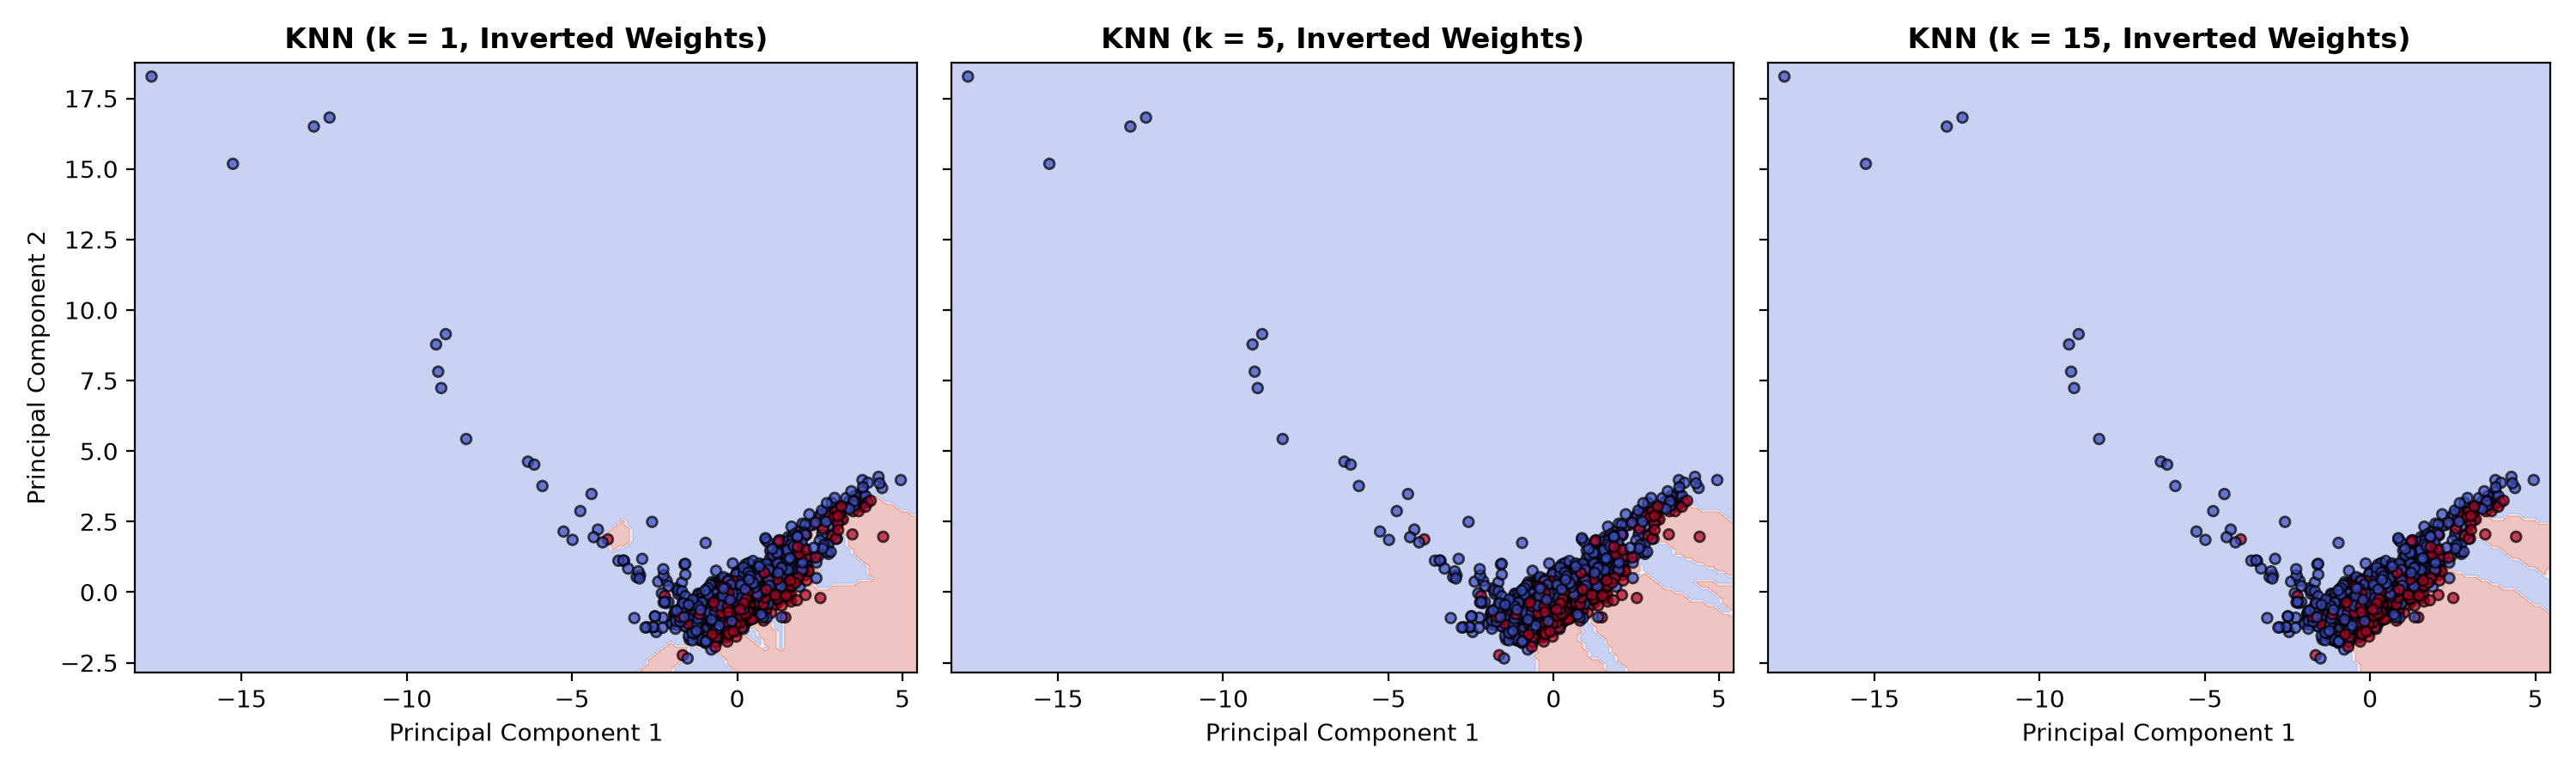
\includegraphics[width=0.95\linewidth]{assets/knn/knn-decision-boundary.png}
  \caption{Visualisasi batas keputusan KNN (\textit{inverted weights}) pada proyeksi dua komponen
  utama pertama untuk variasi nilai $k \in \{1, 5, 15\}$.}
  \label{fig:knn-boundary}
\end{figure}

Visualisasi pada Gambar~\ref{fig:knn-boundary} memperlihatkan dampak pemilihan nilai $k$ terhadap bentuk batas keputusan:
\begin{itemize}
  \item Pada $k=1$, batas keputusan sangat terfragmentasi dan membentuk pulau-pulau kecil di sekitar
        titik pencilan (\textit{overfitting}).
  \item Pada $k=5$, batas keputusan menjadi jauh lebih halus dan kontur pemisah antarkelas terlihat wajar,
        mencapai keseimbangan optimal antara \textit{bias} dan \textit{variance}.
  \item Pada $k=15$, batas keputusan menjadi terlalu menyederhanakan sebaran lokal (\textit{underfitting}),
        sehingga titik-titik minoritas di area perbatasan cenderung terabaikan.
\end{itemize}

\paragraph{Evaluasi Validasi Silang dan Matriks Konfusi.}
Pada pengujian \textit{Stratified 5-Fold Cross Validation} terhadap data latih penuh (27.373 baris)
menggunakan konfigurasi optimal ($k=5$, metrik Euclidean, \textit{inverted weights}, dan ambang
probabilitas $\theta = 0{,}45$), diperoleh rata-rata akurasi sebesar \textbf{0,8395} dan rata-rata
Macro-F1 sebesar \textbf{0,8395} ($\pm 0{,}0032$).

\begin{figure}[htbp]
  \centering
  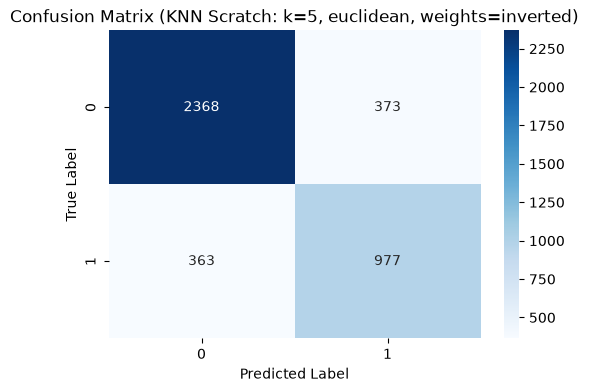
\includegraphics[width=0.48\linewidth]{assets/knn/knn-confusion-matrix.png}
  \caption{Matriks konfusi model KNN final ($k=5$, \textit{inverted weights}, ambang batas probabilitas $\theta = 0{,}45$)
  pada himpunan validasi data asli.}
  \label{fig:knn-cm}
\end{figure}

Matriks konfusi pada Gambar~\ref{fig:knn-cm} menunjukkan bahwa model berhasil mendeteksi pembatalan
(kelas positif 1) secara seimbang dengan \textit{recall} $73\%$ dan \textit{precision} $72\%$,
sementara kelas non-batal (kelas 0) diprediksi dengan presisi $87\%$ dan \textit{recall} $86\%$.
Penyetelan ambang batas pada $\theta = 0{,}45$ secara efektif meningkatkan sensitivitas terhadap pembatalan
tanpa mengorbankan akurasi global secara berlebihan.

\paragraph{Submisi Akhir.}
Model KNN final yang dilatih pada seluruh data latih asli menghasilkan berkas submisi
\texttt{submission\_knn.csv} (6.844 baris data uji). Distribusi hasil prediksi terdiri atas 4.841 sampel
kelas 0 ($70{,}74\%$) dan 2.003 sampel kelas 1 ($29{,}26\%$). Proporsi ini sangat selaras dengan rasio
alami kelas pada data latih asli ($32{,}77\%$ pembatalan), mengonfirmasi bahwa model tidak mengalami bias
ekstrem dan memiliki kemampuan generalisasi yang stabil.

\subsection{Decision Tree Learning (DTL)}

\subsubsection{Implementasi}
Model C4.5 menerima fitur numerik dan kategorikal serta menangani nilai kosong. Pohon dibangun dari akar. Di setiap simpul, model memilih fitur untuk membagi data, lalu mengulangi prosesnya pada tiap cabang.

\paragraph{Penyiapan fitur.}
Fungsi \texttt{prepare\_dtl\_features} menandai nilai numerik negatif, jumlah tamu dewasa nol, durasi menginap nol, dan tanggal yang tidak valid sebagai nilai kosong pada kolom terkait. Nilai kosong dibiarkan agar bobotnya bisa dibagi saat pohon dibentuk. Kode angka untuk kanal pemesanan dan kategori lain tetap diperlakukan sebagai kategori.
Tanggal kedatangan dan pemesanan diubah menjadi jumlah hari sejak 1 Januari 2023 agar bisa dibandingkan. Kami menambahkan total malam, perkiraan biaya menginap, indikator nilai kosong, dan indikator seperti pemesanan tanpa permintaan khusus. Data latih dan data uji diproses secara terpisah.

\paragraph{Pemilihan pemisahan.}
Metode \texttt{fit} pada \texttt{C45DecisionTree} memberi bobot awal 1 pada setiap baris dan memanggil \texttt{\_build\_tree}. Fungsi \texttt{\_find\_split} mencoba ambang dari nilai unik fitur numerik. Setiap ambang $t$ membagi data menjadi $x\leq t$ dan $x>t$. Pada fitur kategorikal, setiap kategori yang muncul mendapat satu cabang.

Gain dihitung dari penurunan entropi pada baris yang nilainya diketahui, lalu dikalikan dengan proporsi bobot baris tersebut. Gain ratio membagi gain dengan \textit{split information}, yaitu entropi dari pembagian bobot ke tiap cabang serta kelompok nilai kosong. Dari kandidat terbaik tiap fitur, model memilih gain ratio tertinggi di antara kandidat dengan gain setidaknya sebesar rata-rata.

\paragraph{Nilai kosong dan prediksi.}
Di \texttt{\_build\_tree}, baris yang nilainya kosong dimasukkan ke semua cabang. Bagian bobot yang diterima setiap cabang mengikuti proporsi bobot dari baris yang nilainya diketahui.

\noindent\begin{minipage}{\linewidth}
\begin{lstlisting}
for branch, rows in groups.items():
    fraction = weights[rows].sum() / known_weight
    selected = rows | missing
    child_weights = weights[selected]
    child_weights[missing[selected]] *= fraction
    child = _build_tree(
        X[selected],
        y[selected],
        child_weights,
        features,
        n_classes,
        next_depth,
        min_branch_weight,
    )
    node["children"][branch] = (child, fraction)
\end{lstlisting}
\end{minipage}

\texttt{predict\_proba} mengikuti cabang yang sesuai hingga mencapai daun. Saat nilainya kosong atau kategorinya belum muncul pada simpul itu, probabilitas dari tiap cabang dirata-ratakan sesuai bobot. Pada v4, kedalaman maksimum adalah 16. Sebuah pemisahan hanya dipakai jika minimal dua cabang masing-masing punya bobot data yang diketahui sebesar 7 atau lebih. \texttt{predict} memberi label batal jika probabilitas kelas 1 mencapai $0{,}48$.

\subsubsection{Hasil dan Perbandingan dengan scikit-learn}
Ketiga model diuji pada 5.475 baris validasi yang sama. Data dibagi secara terstratifikasi (80\% latih dan 20\% validasi) dengan \texttt{random\_state=824}. Metrik utama yang dipakai adalah Macro F1, yaitu rata-rata F1 kelas batal dan tidak batal.

Pembanding \texttt{DecisionTreeClassifier} memakai kriteria \texttt{entropy} dan kedalaman maksimum 16. Dari tiga nilai \texttt{ccp\_alpha} yang dicoba, $0{,}0005$ memberi Macro F1 validasi tertinggi. Median, modus, dan pengodean \textit{one-hot} ditentukan dari data latih, lalu dipakai pada data validasi.

\begin{table}[!htbp]
  \centering
  \caption{Hasil validasi DTL pada pemisahan 80:20.}
  \label{tab:dtl-validation}
  \begin{tabular}{@{}lrr@{}}
    \toprule
    Model & Akurasi & Macro F1 \\
    \midrule
    C4.5 v3 & 0,85753 & 0,83744 \\
    C4.5 v4 & 0,85717 & \textbf{0,83842} \\
    scikit-learn & 0,85425 & 0,83183 \\
    \bottomrule
  \end{tabular}
\end{table}

Macro F1 v4 naik sekitar 0,10 poin persentase dari v3. Akurasi keduanya hampir sama (Tabel~\ref{tab:dtl-validation}). Pada Gambar~\ref{fig:dtl-confusion}, v4 mengenali 1.414 pembatalan dan scikit-learn mengenali 1.339. Jumlah pemesanan yang keliru diprediksi batal adalah 402 pada v4 dan 343 pada scikit-learn.

\begin{figure}[!htbp]
  \centering
  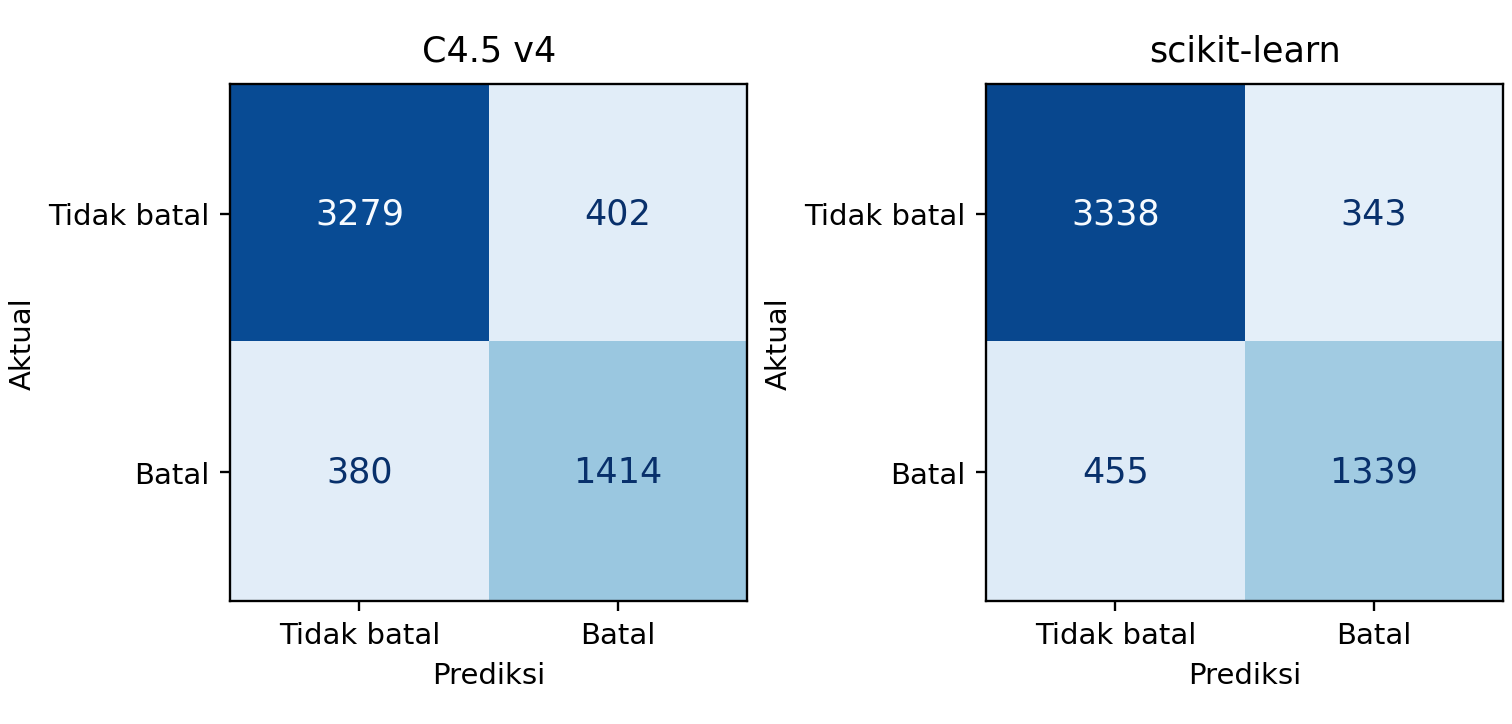
\includegraphics[width=0.94\linewidth]{assets/dtl/dtl_confusion.png}
  \caption{Matriks kebingungan C4.5 v4 dan scikit-learn pada data validasi yang sama.}
  \label{fig:dtl-confusion}
\end{figure}

Untuk submisi, v4 dilatih ulang pada seluruh data latih. Prediksi sebelum dan sesudah model disimpan dan dimuat kembali identik. CSV berisi 6.844 prediksi dengan urutan ID sesuai templat submisi. Skor publik Kaggle untuk v4 adalah 0,84191 (Macro F1).

\subsubsection{Visualisasi Pohon}
Gambar~\ref{fig:dtl-tree} menampilkan pohon v4 yang dipakai untuk submisi. Fungsi \texttt{plot\_dtl\_tree} menelusuri pohon per tingkat dari akar. Pada simpul yang sama, cabang berbobot lebih besar digambar dulu. Parameter \texttt{top\_n} membatasi jumlah cabang yang terlihat. Di gambar ini batasnya 10.
Pada akar, model membagi pemesanan lewat \texttt{days\_before\_arrival}. Bobot kelas batal sekitar 24\% pada pemesanan yang dibuat paling lama 152 hari sebelum kedatangan dan 70\% pada pemesanan yang dibuat lebih awal.

\begin{figure}[!htbp]
  \centering
  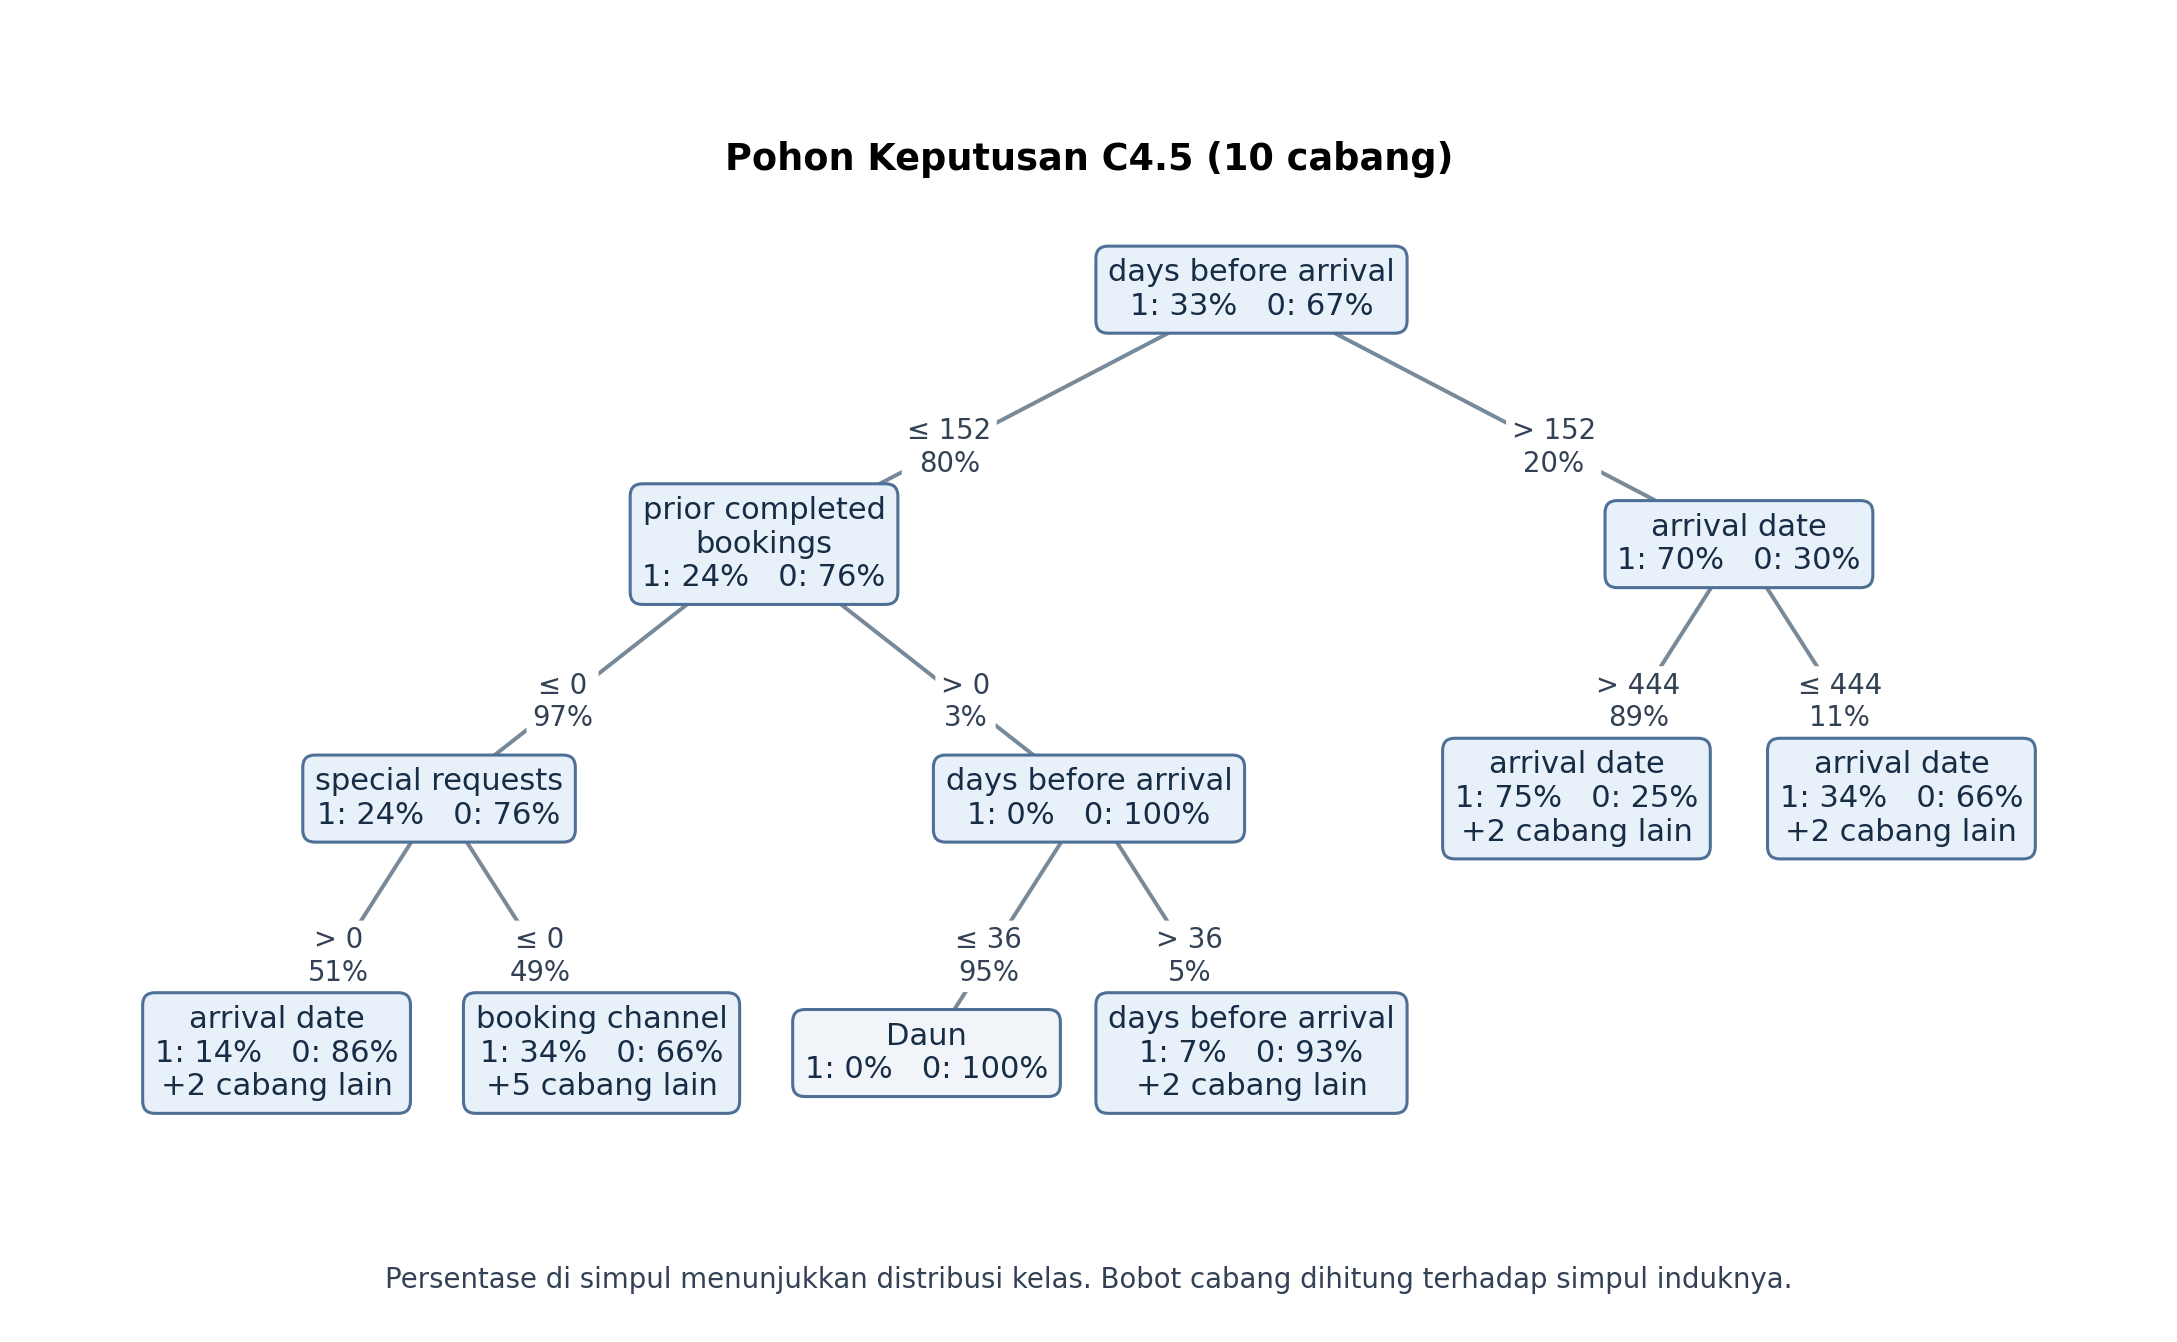
\includegraphics[width=\linewidth]{assets/dtl/dtl_tree.png}
  \caption{Sepuluh cabang awal pohon C4.5 v4. Kelas 0 berarti tidak batal dan kelas 1 berarti batal.}
  \label{fig:dtl-tree}
\end{figure}

\subsection{Logistic Regression}

Logistic Regression biner memodelkan probabilitas bersyarat kelas positif
$y = 1$ (pemesanan dibatalkan) terhadap fitur masukan $x \in \mathbb{R}^d$
melalui kombinasi linear (\textit{log-odds}) $z = b_0 + \sum_{j=1}^d b_j x_j = b^\top \tilde{x}$
dengan $\tilde{x} = [1, x^\top]^\top$ dan fungsi aktivasi sigmoid (Khodra, 2021):
\[
  P(y = 1 \mid x) = \sigma(z) = \frac{1}{1 + e^{-z}}.
\]
Pelatihan parameter $b$ dilakukan berdasarkan prinsip \textit{Maximum Likelihood
Estimation} (MLE) dengan memaksimumkan \textit{Log Joint Conditional Likelihood}
(LCL), yang ekuivalen dengan meminimalkan rata-rata \textit{negative log-loss}
ditambah suku regularisasi $R(b_{1:d})$ (Khodra, 2021):
\[
  \mathcal{L}(b) = -\frac{1}{n}\sum_{i=1}^{n} \Big[y_i \log p_i + (1 - y_i)\log(1 - p_i)\Big] + R(b_{1:d}),
\]
dengan $p_i = \sigma(b^\top \tilde{x}_i)$. Suku penalti hanya dikenakan pada bobot
fitur $w = b_{1:d}$ (tidak pada \textit{bias} $b_0$) untuk tiga varian:
\[
  R_{\text{L1}}(w) = \lambda \sum_{j=1}^{d} |w_j|, \qquad
  R_{\text{L2}}(w) = \frac{\lambda}{2} \sum_{j=1}^{d} w_j^2, \qquad
  R_{\text{EN}}(w) = \lambda \left( r \sum_{j=1}^{d} |w_j| + \frac{1 - r}{2} \sum_{j=1}^{d} w_j^2 \right),
\]
dengan $\lambda$ adalah \texttt{reg\_lambda} dan $r \in [0, 1]$ adalah
\texttt{l1\_ratio}.

\subsubsection{Implementasi}

Implementasi \textit{from scratch} berada pada berkas
\texttt{src/models/logistic\_regression.py} (337 baris) dan diintegrasikan
dengan antarmuka tim melalui kelas \texttt{LogisticRegression(BaseModel)},
konfigurasi \texttt{DEFAULT\_LOGREG\_CONFIGS}, serta
\texttt{get\_logreg\_preprocessing\_config()}. Pipeline \textit{preprocessing}
mengaktifkan standarisasi numerik, SMOTE pada himpunan latih, seleksi fitur, dan
PCA agar skala fitur seragam dan gradien tetap stabil.

Komponen utama di dalam kelas \texttt{LogisticRegression} meliputi:
\begin{itemize}
  \item \texttt{\_sigmoid}, \texttt{\_add\_intercept}, \texttt{log\_odds},
        \texttt{\_compute\_lcl}, \texttt{\_compute\_penalty}, dan
        \texttt{\_regularization\_grad}: melakukan pemotongan numerik
        (\textit{clipping}) pada logit $[-500, 500]$ dan probabilitas
        $[10^{-15}, 1 - 10^{-15}]$ untuk mencegah \textit{overflow}/\texttt{log(0)},
        serta menghitung nilai dan turunan penalti L1, L2, dan Elastic Net.
  \item \texttt{\_fit\_sga} dan \texttt{\_fit\_adam}: menyediakan dua metode
        optimasi, yakni \textit{Stochastic Gradient Ascent} (SGA) sesuai materi
        kuliah (Khodra, 2021) dan \textit{mini-batch Adam} sebagai metode
        optimasi tambahan (Kingma dan Ba, 2015). Keduanya mencatat riwayat
        \texttt{lcl\_history\_} serta \texttt{loss\_history\_} pada tiap
        \textit{epoch} melalui \texttt{\_record\_epoch} dan berhenti otomatis
        apabila perubahan \textit{loss} lebih kecil dari \texttt{tol}.
  \item \texttt{fit}, \texttt{predict\_proba}, \texttt{predict}, serta
        \texttt{save}/\texttt{load}: memetakan label target ke $\{0, 1\}$,
        memprediksi kelas dengan ambang \texttt{threshold} (bawaan $0{,}5$), dan
        mendukung serialisasi berbasis \texttt{joblib} (dengan cadangan
        \texttt{pickle}).
\end{itemize}

Pada SGA, pembaruan dilakukan secara sekuensial per sampel ($\tilde{x}_i$),
sehingga lintasan gradien cenderung berosilasi dan membutuhkan iterasi baris
dalam Python. Sebaliknya, \textbf{Adam} (\textit{Adaptive Moment Estimation})
mengoptimasi proses pelatihan lewat empat mekanisme (Kingma dan Ba, 2015):
(1) menghitung gradien secara vektorisasi per \textit{mini-batch} berukuran 256;
(2) mempertahankan momentum orde pertama $m_t = \beta_1 m_{t-1} + (1 - \beta_1) g_t$
($\beta_1 = 0{,}9$) agar arah pembaruan lebih halus; (3) mempertahankan estimasi
variansi gradien orde kedua $v_t = \beta_2 v_{t-1} + (1 - \beta_2) g_t^2$
($\beta_2 = 0{,}999$) untuk menyesuaikan ukuran langkah adaptif tiap parameter; dan
(4) menerapkan koreksi bias $\hat{m}_t, \hat{v}_t$ sehingga konvergensi awal
lebih stabil tanpa menuntut penyetelan \textit{learning rate} yang ketat.

\begin{lstlisting}
def _regularization_grad(self):
    w = self.b_[1:]
    if self.penalty == "l1":
        return self.reg_lambda * np.sign(w)
    if self.penalty == "l2":
        return self.reg_lambda * w
    if self.penalty == "elasticnet":
        return self.reg_lambda * (self.l1_ratio * np.sign(w) + (1.0 - self.l1_ratio) * w)
    return np.zeros_like(w)

def _fit_sga(self, X_bias, y_bin):
    rng = np.random.default_rng(self.random_state)
    use_reg = self.penalty not in (None, "none") and self.reg_lambda > 0.0
    for epoch in range(1, self.max_iter + 1):
        for idx in (rng.permutation(len(X_bias)) if self.shuffle else range(len(X_bias))):
            x_i = X_bias[idx]
            p_i = self._sigmoid(np.dot(self.b_, x_i))
            self.b_ += self.learning_rate * (y_bin[idx] - p_i) * x_i
            if use_reg:
                self.b_[1:] -= self.learning_rate * self._regularization_grad()
        if self._record_epoch(epoch, X_bias, y_bin):
            break

def _fit_adam(self, X_bias, y_bin):
    m, v = np.zeros(X_bias.shape[1]), np.zeros(X_bias.shape[1])
    t_step = 0
    for epoch in range(1, self.max_iter + 1):
        ...
        t_step += 1
        m = self.beta1 * m + (1.0 - self.beta1) * grad
        v = self.beta2 * v + (1.0 - self.beta2) * (grad ** 2)
        m_hat = m / (1.0 - self.beta1 ** t_step)
        v_hat = v / (1.0 - self.beta2 ** t_step)
        self.b_ -= self.learning_rate * m_hat / (np.sqrt(v_hat) + self.eps)
\end{lstlisting}

\subsubsection{Hasil dan Perbandingan dengan scikit-learn}

Eksperimen lengkap dijalankan melalui
\texttt{notebooks/logistic\_regression\_experiment.ipynb} menggunakan pembagian
data validasi 15\% (\texttt{random\_state=824}). Evaluasi 5-\textit{fold
Stratified Cross-Validation} pada himpunan latih (mencakup seluruh kombinasi
regularisasi dan \textit{optimizer} pada \texttt{DEFAULT\_LOGREG\_CONFIGS})
dirangkum pada Tabel~\ref{tab:logreg-cv}.

\begin{table}[htbp]
  \centering
  \caption{Hasil 5-\textit{Fold Stratified Cross-Validation} Logistic Regression \textit{from scratch}.}
  \label{tab:logreg-cv}
  \footnotesize
  \begin{tabular}{llccc}
    \toprule
    \textbf{Optimizer} & \textbf{Regularisasi} & \textbf{Epoch / LR} & \textbf{Mean Akurasi} & \textbf{Mean Macro-F1} \\
    \midrule
    SGA  & Tanpa penalti (\texttt{None}) & 20 / 0,01 & 0,75147 & 0,75121 $\pm$ 0,00402 \\
    SGA  & L1 ($\lambda = 10^{-4}$) & 20 / 0,01 & 0,75083 & 0,75056 $\pm$ 0,00445 \\
    SGA  & L2 ($\lambda = 10^{-4}$) & 20 / 0,01 & 0,74999 & 0,74971 $\pm$ 0,00433 \\
    SGA  & Elastic Net ($\lambda = 10^{-4}, r = 0{,}5$) & 20 / 0,01 & 0,74977 & 0,74948 $\pm$ 0,00388 \\
    Adam & L2 ($\lambda = 10^{-4}$, \texttt{bs}=256) & 30 / 0,02 & 0,75064 & 0,75051 $\pm$ 0,00496 \\
    Adam & Elastic Net ($\lambda = 10^{-4}, r = 0{,}5$) & 30 / 0,02 & 0,75093 & 0,75079 $\pm$ 0,00502 \\
    \bottomrule
  \end{tabular}
\end{table}

Selisih antar-konfigurasi pada validasi silang sangat tipis ($< 0{,}002$ pada
\textit{macro-F1}) karena fitur masukan sudah melalui \texttt{SelectKBest} dan
PCA sehingga dimensi fitur lebih kompak dan ortogonal. Konfigurasi terbaik dari
CV (\texttt{SGA}, \texttt{penalty=None}, \texttt{lr=0,01}, 20 \textit{epoch})
kemudian dilatih ulang hanya pada baris latih asli (\texttt{fit\_orig\_only=True})
dan diuji pada 4.081 baris validasi asli (2.741 kelas 0 dan 1.340 kelas 1)
melawan \texttt{sklearn.linear\_model.LogisticRegression(max\_iter=1000)}.
Hasil perbandingan disajikan pada Tabel~\ref{tab:logreg-sklearn} dan
Gambar~\ref{fig:logreg-eval}.

\begin{table}[htbp]
  \centering
  \caption{Perbandingan Logistic Regression \textit{from scratch} dan \texttt{scikit-learn} pada 4.081 sampel validasi asli.}
  \label{tab:logreg-sklearn}
  \footnotesize
  \begin{tabular}{lcccc}
    \toprule
    \textbf{Model} & \textbf{Akurasi} & \textbf{Presisi} & \textbf{Recall} & \textbf{Macro-F1} \\
    \midrule
    \texttt{LogisticRegression} (Scratch - SGA) & 0,77922 & 0,73833 & 0,50746 & 0,72441 \\
    \texttt{LogisticRegression} (Scikit-Learn)  & 0,78069 & 0,73446 & 0,52015 & 0,72830 \\
    \bottomrule
  \end{tabular}
\end{table}

\begin{figure}[htbp]
  \centering
  \begin{minipage}{0.46\textwidth}
    \centering
    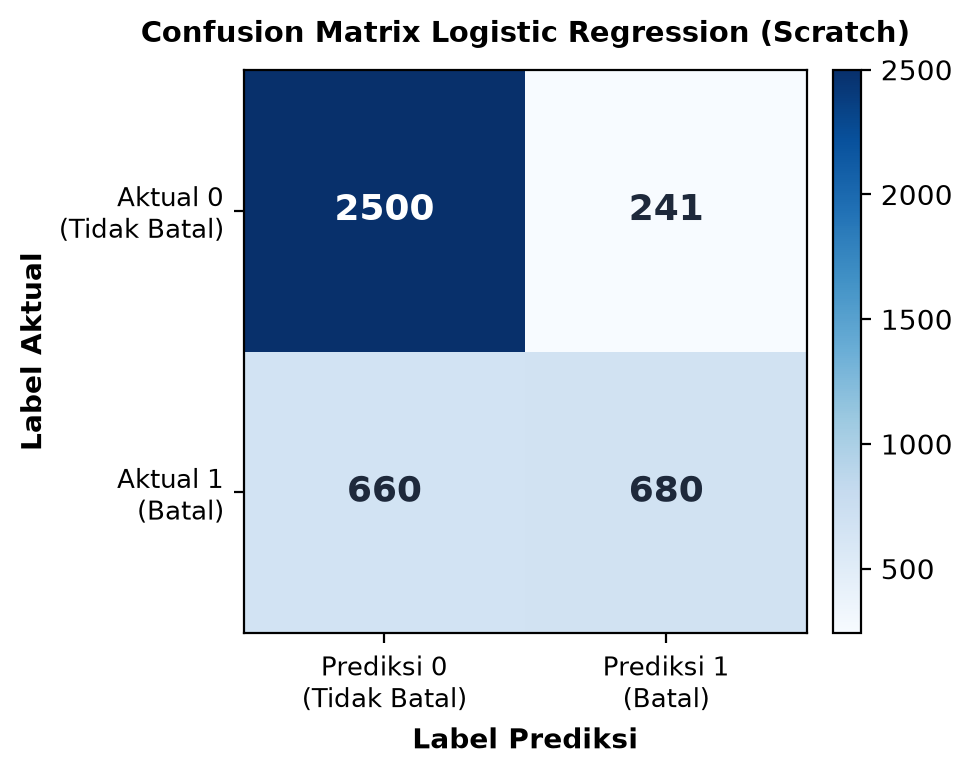
\includegraphics[width=\linewidth]{assets/logreg/logreg-cm.png}\\
    (a) \textit{Confusion matrix} model terbaik
  \end{minipage}\hfill
  \begin{minipage}{0.51\textwidth}
    \centering
    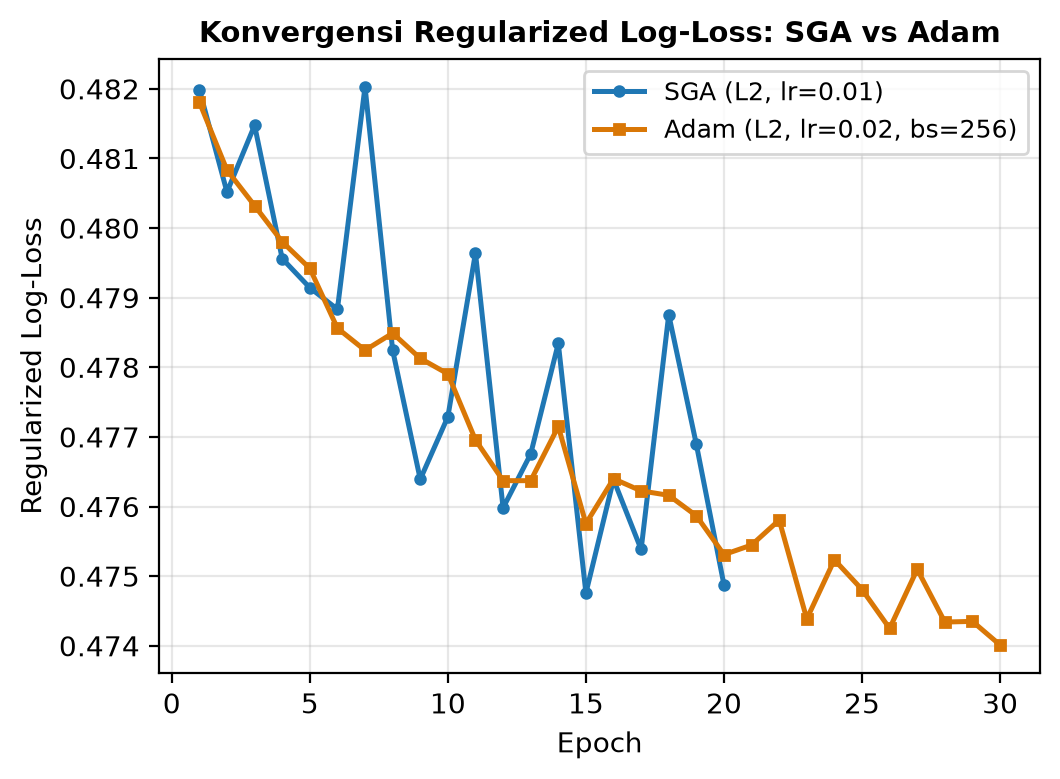
\includegraphics[width=\linewidth]{assets/logreg/logreg-loss.png}\\
    (b) Kurva konvergensi \textit{log-loss} SGA vs Adam
  \end{minipage}
  \caption{Evaluasi \textit{confusion matrix} pada himpunan validasi asli dan perbandingan konvergensi SGA terhadap mini-batch Adam.}
  \label{fig:logreg-eval}
\end{figure}

Secara kuantitatif, implementasi \textit{from scratch} sangat mendekati
pustaka referensi: selisih akurasi hanya 0,00147, \textit{macro-F1} berselisih
0,00389, tingkat kesepakatan prediksi (\textit{prediction agreement}) mencapai
\textbf{97,35\%}, dan \textit{cosine similarity} antara vektor bobot fitur kedua
model mencapai \textbf{0,99743}. Perbedaan kecil tersebut wajar karena
\texttt{scikit-learn} menggunakan \textit{solver} kuasi-Newton \texttt{lbfgs}
dengan regularisasi L2 bawaan hingga konvergen penuh, sedangkan model
\textit{from scratch} berhenti pada 20 \textit{epoch} SGA.

Dari Gambar~\ref{fig:logreg-eval}(a), diperoleh $\text{TN} = 2.500$,
$\text{FP} = 241$, $\text{FN} = 660$, dan $\text{TP} = 680$. Model mengenali
kelas mayoritas (tidak batal) dengan sangat baik (\textit{recall} $0{,}91$,
F1 $0{,}85$), tetapi lebih konservatif pada kelas positif (\textit{recall}
$0{,}51$, F1 $0{,}60$) karena distribusi kelas tidak seimbang dan pemisahan
antar-kelas di ruang fitur PCA bersifat non-linear. Sementara itu, perbandingan
SGA vs Adam berpenalti L2 ($\lambda = 10^{-4}$) pada Gambar~\ref{fig:logreg-eval}(b)
menunjukkan bahwa mini-batch Adam (30 \textit{epoch}) jauh lebih cepat secara
komputasi (\textbf{0,064 detik} dibanding \textbf{1,602 detik} pada SGA
20 \textit{epoch}, atau $\sim 25\times$ lebih cepat berkat vektorisasi batch) dan
mencapai \textit{regularized log-loss} latih lebih rendah (\textbf{0,47401} vs
\textbf{0,47487}), dengan akurasi validasi yang tetap sebanding (0,77162 vs
0,77824).

Terakhir, verifikasi penyimpanan model ke \texttt{output/logreg.pkl}
(berukuran \textbf{1,13 KB}) mengonfirmasi bobot hasil \textit{load} identik
dengan model sebelum disimpan. Inferensi pada seluruh 6.844 baris data uji di
\texttt{output/submission\_logreg.csv} menghasilkan distribusi prediksi
5.268 kelas 0 (76,97\%) dan 1.576 kelas 1 (23,03\%) yang konsisten dengan sifat
konservatif model terhadap kelas positif.

\subsection{Support Vector Machine (SVM)}

Support Vector Machine (SVM) mencari \textit{hyperplane} pemisah yang memaksimalkan
\textit{margin}, yaitu jarak terkecil antara bidang pemisah dan titik-titik data
terdekat (\textit{support vector}). Untuk data yang tidak sepenuhnya terpisah
secara linear, digunakan \textit{soft margin} dengan variabel \textit{slack}
$\xi_i \ge 0$ dan parameter regularisasi $C$:
\[
\min_{w,b,\xi}\ \frac{1}{2}\lVert w \rVert^2 + C\sum_{i=1}^n \xi_i
\quad \text{s.t.}\quad y_i(w^\top x_i + b) \ge 1 - \xi_i,\ \xi_i \ge 0 .
\]
Bentuk \textit{dual}-nya adalah
\[
\max_{\alpha}\ \sum_{i=1}^n \alpha_i
- \frac{1}{2}\sum_{i=1}^n\sum_{j=1}^n \alpha_i\alpha_j y_i y_j K(x_i,x_j),
\quad
\text{s.t.}\quad 0 \le \alpha_i \le C,\ \sum_{i=1}^n \alpha_i y_i = 0,
\]
sehingga fungsi keputusan hanya bergantung pada \textit{support vector}:
\[
f(x) = \sum_{i \in SV}\alpha_i y_i K(x_i,x) + b .
\]
\textit{Kernel trick} memungkinkan SVM memisahkan data non-linear tanpa
menghitung pemetaan fitur secara eksplisit. Pada tugas ini SVM diimplementasikan
dari nol untuk klasifikasi biner target \texttt{is\_canceled} pada dataset hotel
(27.373 baris latih, 6.844 baris uji, 32,77\% kelas positif).

\subsubsection{Implementasi}

Implementasi SVM dari nol berada pada paket \texttt{src/svm/} dan dipisahkan
menjadi empat komponen utama:
\begin{itemize}
  \item \texttt{kernels.py}: fungsi kernel \textit{linear}, \textit{polinomial},
        dan RBF, beserta resolusi nilai $\gamma$;
  \item \texttt{smo.py}: \textit{solver} Sequential Minimal Optimization (SMO)
        dengan pemilihan \textit{working set} orde kedua dan \textit{cache} kernel;
  \item \texttt{model.py}: kelas \texttt{SVM} yang menyatukan kernel, solver,
        penyimpanan \textit{support vector}, serta prediksi;
  \item \texttt{features.py} dan \texttt{data.py}: rekayasa fitur (target
        encoding, fitur interaksi, penskalaan \textit{robust}) dan pemuatan data.
\end{itemize}

\paragraph{Fungsi kernel.}
Tiga kernel yang didukung adalah kernel linear, polinomial, dan RBF
(\textit{Radial Basis Function}):
\[
K_{\text{linear}}(x,z)=x^\top z,\qquad
K_{\text{poli}}(x,z)=(\gamma\,x^\top z + r)^d,\qquad
K_{\text{RBF}}(x,z)=\exp(-\gamma\lVert x-z\rVert^2).
\]
Nilai $\gamma$ dapat berupa bilangan positif, \texttt{"auto"} $=1/d$, atau
\texttt{"scale"} $=1/(d\cdot\mathrm{Var}(X))$ seperti pada scikit-learn. Agar
stabil secara numerik, kernel RBF menghitung matriks jarak secara \textit{block}
untuk data besar dan memotong nilai negatif akibat galat pembulatan.
\begin{lstlisting}
def rbf_kernel(X, Y=None, gamma=1.0):
    X, Y = _check(X, Y)
    X2 = np.einsum("ij,ij->i", X, X)
    Y2 = np.einsum("ij,ij->i", Y, Y)
    D = X2[:, None] + Y2[None, :] - 2.0 * (X @ Y.T)
    np.maximum(D, 0.0, out=D)
    return np.exp(-gamma * D)
\end{lstlisting}

\paragraph{Solver SMO.}
Optimasi dual diselesaikan dengan SMO yang memperbarui dua koefisien
$\alpha_i,\alpha_j$ pada setiap langkah. Pasangan dipilih menggunakan informasi
orde kedua (Fan, Chen, dan Lin, 2005):
\[
(i,j) = \arg\max_{(i,j)}\ \frac{(E_j - E_i)^2}
{K_{ii} + K_{jj} - 2K_{ij}},
\qquad E_i = f(x_i) - y_i,
\]
dengan batas $L \le \alpha_j \le H$ yang bergantung pada kesamaan label dan
nilai $\alpha_i,\alpha_j$ saat ini. Setelah $\alpha_j$ diperbarui,
$\alpha_i$ dihitung agar kendala $\sum_i \alpha_i y_i = 0$ tetap terpenuhi,
lalu \textit{bias} $b$ diperbarui berdasarkan KKT. Solver berhenti ketika
pelanggaran KKT $\max_{i\in I_{\text{low}}} E_i - \min_{j\in I_{\text{up}}} E_j$
sudah di bawah toleransi. Representasi matriks kernel dikelola
\texttt{KernelProvider}: jika ukuran matriks muat di \textit{budget} memori,
matriks penuh disimpan; jika tidak, baris kernel dihitung malas dan disimpan
dalam \textit{LRU cache}.
\begin{lstlisting}
eta = 2.0 * Kij - Kii - Kjj
aj_new = aj - yj * (Ei - Ej) / eta
aj_new = min(max(aj_new, L), H)
ai_new = ai + yi * yj * (aj - aj_new)
...
errors += yi * dai * row_i
errors += yj * daj * provider.row(j)
errors += b_new - b
\end{lstlisting}

\paragraph{Kelas SVM.}
Kelas \texttt{SVM} mengikuti antarmuka \texttt{fit}/\texttt{predict}. Saat
\textit{fit}, label dipetakan ke $\{-1,+1\}$, $\gamma$ diresolusikan, matriks
kernel dibangun, SMO dijalankan, dan \textit{support vector} disimpan
($\alpha_i > 10^{-5}$). Untuk kernel linear, vektor bobot $w$ dan lebar
\textit{margin} juga dihitung. Prediksi menggunakan tanda dari
\texttt{decision\_function}. Model mendukung penyimpanan \texttt{joblib} dan
diverifikasi \textit{round-trip}-nya agar prediksi identik sebelum dan sesudah
disimpan.
\begin{lstlisting}
class SVM:
    def fit(self, X, y):
        ...
        y_pm = np.where(y == classes[1], 1.0, -1.0)
        gamma = resolve_gamma(self.gamma, X, self.kernel)
        provider = KernelProvider(X, self.kernel, self.degree,
                                  gamma, self.coef0, self.cache_size_mb)
        result = solve_smo(provider, y_pm, float(self.C),
                           tol=self.tol, max_iter=self.max_iter)
        sv = result.alpha > 1e-5
        self.support_vectors_ = X[sv]
        self.dual_coef_ = (result.alpha[sv] * y_pm[sv]).reshape(1, -1)
        self.intercept_ = np.array([result.b])
        return self

    def decision_function(self, X):
        K = kernel_matrix(X, self.support_vectors_, self.kernel,
                          self.degree, self.gamma_, self.coef0)
        return K @ self.dual_coef_[0] + self.intercept_[0]
\end{lstlisting}

\paragraph{Pengujian.}
Implementasi diverifikasi melalui \texttt{tests/test\_svm.py}. Fungsi kernel
dibandingkan langsung dengan \texttt{sklearn.metrics.pairwise} (toleransi
$10^{-12}$), sedangkan perilaku model diuji pada data terpisah linear, data XOR,
batas $\alpha \in [0,C]$, pemenuhan KKT, penolakan klasifikasi multikelas,
reproduksibilitas, dan kesamaan prediksi setelah serialisasi. Pengujian juga
membandingkan hasil dengan \texttt{sklearn.svm.SVC} pada data \textit{blob};
akurasi keduanya berbeda kurang dari 0,15 dengan kesepakatan tanda prediksi
di atas 85\%.

\subsubsection{Hasil dan Perbandingan dengan scikit-learn}

Perbandingan dilakukan secara adil: model \textit{from scratch} dan
\texttt{sklearn.svm.SVC} dilatih pada subset terstratifikasi yang sama
(5.000 baris), dengan fitur, \textit{split} validasi, dan hiperparameter identik
($C=1$, $\gamma=$ \texttt{scale}, $d=3$, $r=0$, toleransi $10^{-3}$). Metrik
dihitung hanya pada baris validasi asli (tanpa data sintetis). Hasilnya
dirangkum pada Tabel~\ref{tab:svm-kernel}.

\begin{table}[htbp]
  \centering
  \caption{Perbandingan SVM \textit{from scratch} dan scikit-learn pada subset
  5.000 baris untuk tiga kernel. SV = jumlah \textit{support vector}.}
  \label{tab:svm-kernel}
  \footnotesize
  \begin{tabular}{llcccccc}
    \toprule
    Kernel & Model & Akurasi & Macro-F1 & F1 kelas 1 & SV & Latih (s) & Prediksi (s) \\
    \midrule
    Linear  & Scratch & 0,7601 & 0,7387 & 0,6639 & 2974 & 8,08 & 0,019 \\
            & sklearn & 0,7596 & 0,7383 & 0,6635 & 2975 & 0,50 & 0,207 \\
    \midrule
    Poli ($d=3$) & Scratch & 0,7508 & 0,7302 & 0,6556 & 3225 & 3,47 & 0,355 \\
            & sklearn & 0,7506 & 0,7300 & 0,6554 & 3224 & 0,42 & 0,241 \\
    \midrule
    RBF     & Scratch & 0,7687 & 0,7454 & 0,6683 & 2905 & 1,82 & 0,234 \\
            & sklearn & 0,7687 & 0,7454 & 0,6683 & 2905 & 0,35 & 0,316 \\
    \bottomrule
  \end{tabular}
\end{table}

Secara kuantitatif, hasil \textit{from scratch} hampir identik dengan
scikit-learn. Untuk kernel linear dan polinomial, selisih akurasi hanya
$0{,}0005$ dan $0{,}0002$; untuk RBF seluruh metrik sama hingga empat angka
desimal. Jumlah \textit{support vector} berbeda paling banyak satu titik
(2975 berbanding 2974 pada kernel linear). Kesepakatan tanda skor keputusan
mencapai 0,9995 (linear), 0,9998 (polinomial), dan 1,0000 (RBF), dengan korelasi
skor $\approx 1{,}0$. Perbedaan kecil tersebut wajar karena SMO berhenti pada
toleransi KKT yang sama tetapi urutan pembaruan pasangan $\alpha$ dan
pembulatan \textit{bias} dapat berbeda; keduanya menyelesaikan masalah
optimasi dual yang sama.

Dari sisi performa, kernel RBF memberikan \textit{macro-F1} terbaik
(0,7454), diikuti linear (0,7387) dan polinomial (0,7302). Hal ini masuk akal
karena hubungan antarfitur dan target cenderung non-linear, sementara kernel
polinomial derajat tiga dengan $\gamma=$ \texttt{scale} pada data ini lebih
sulit dikalibrasi. Pemilihan kernel RBF konsisten dengan hasil eksperimen
lanjutan.

Gambar~\ref{fig:svm-margin} memperlihatkan ilustrasi batas keputusan dan
\textit{margin} pada dua komponen utama pertama. Ilustrasi ini hanya bertujuan
visual: model pada gambar dilatih pada bidang 2D, bukan model 9--116 dimensi
yang dipakai untuk submisi. Terlihat bahwa kernel linear menghasilkan batas
berupa garis lurus, sedangkan kernel RBF mampu membentuk batas melengkung dan
mengelilingi awan data dengan lebih baik.

\begin{figure}[htbp]
  \centering
  \begin{minipage}{0.32\textwidth}
    \centering
    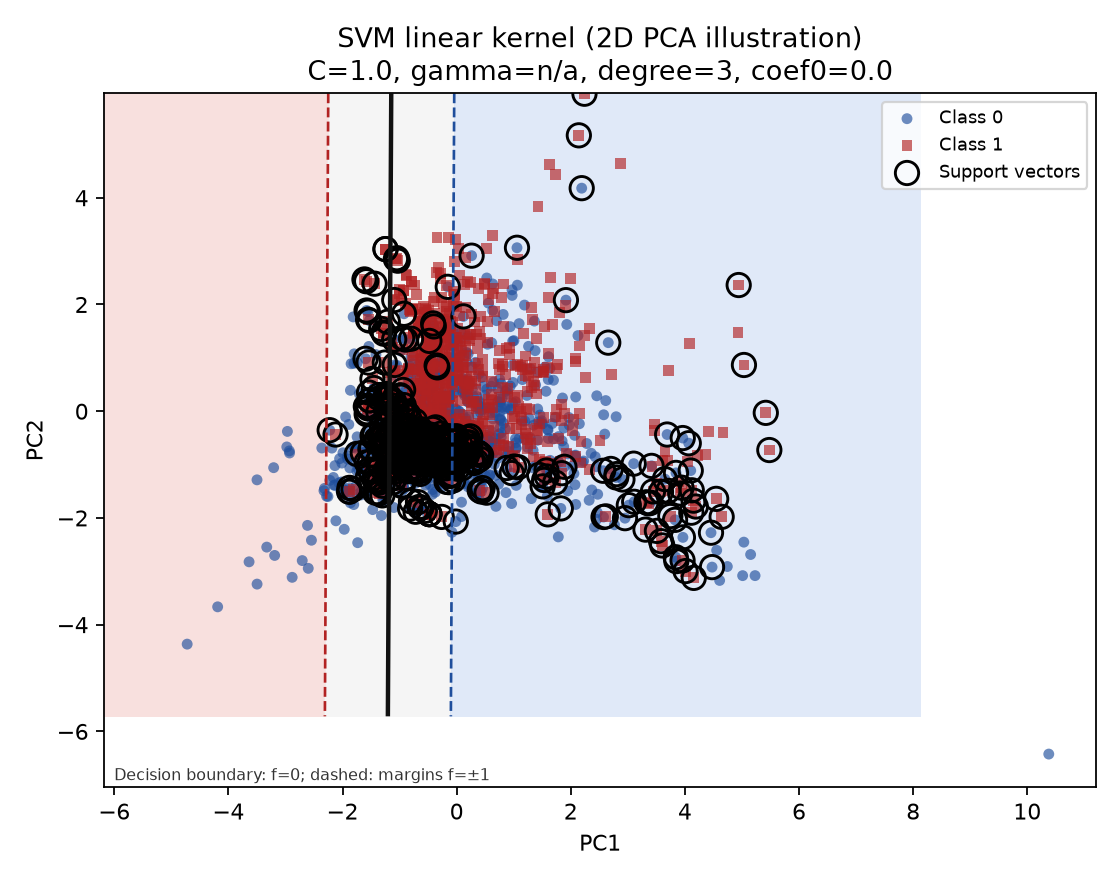
\includegraphics[width=\linewidth]{assets/svm/svm-margin-linear.png}\\
    (a) Linear
  \end{minipage}\hfill
  \begin{minipage}{0.32\textwidth}
    \centering
    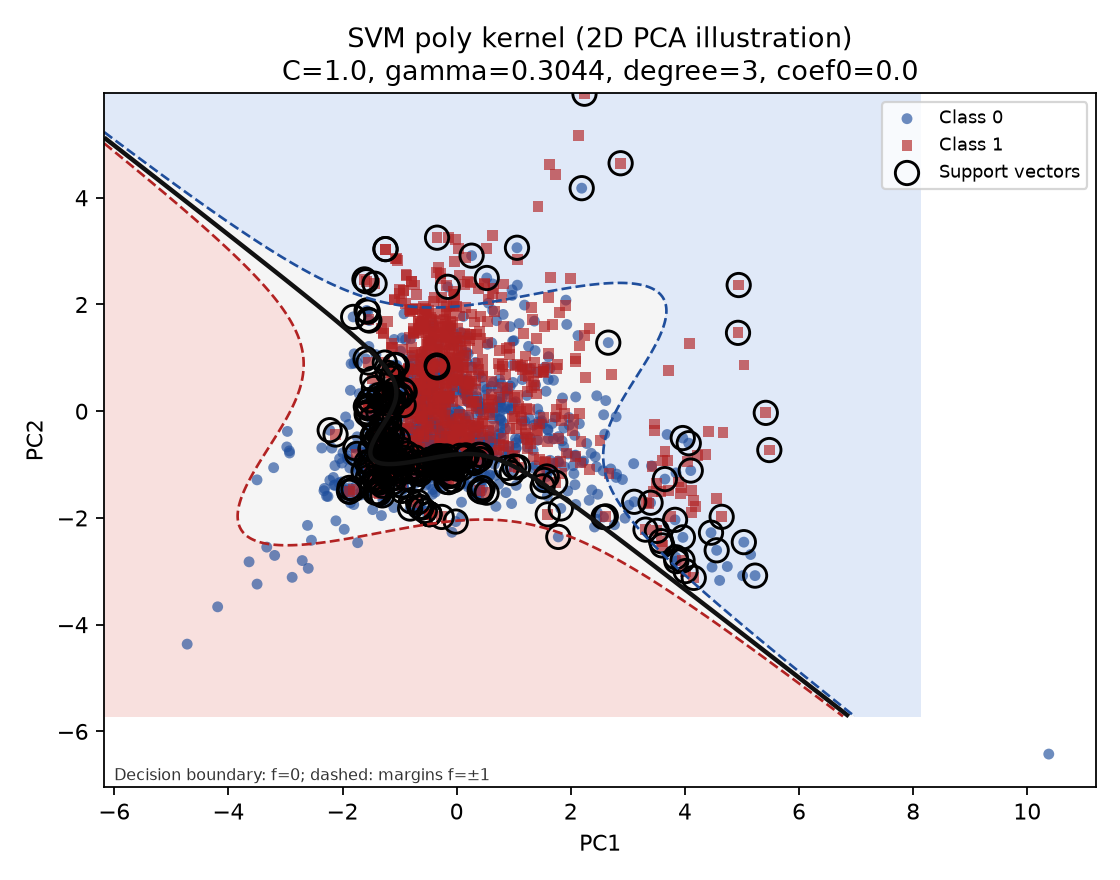
\includegraphics[width=\linewidth]{assets/svm/svm-margin-poly.png}\\
    (b) Polinomial ($d=3$)
  \end{minipage}\hfill
  \begin{minipage}{0.32\textwidth}
    \centering
    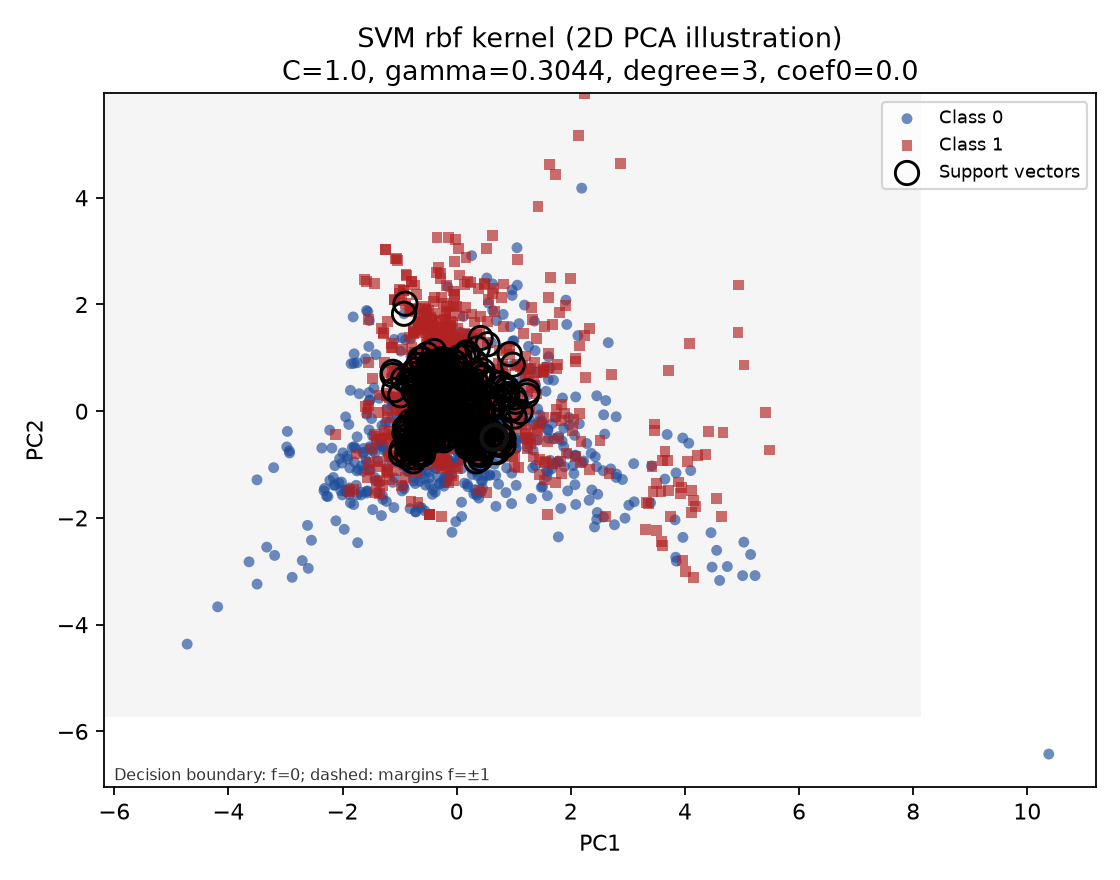
\includegraphics[width=\linewidth]{assets/svm/svm-margin-rbf.png}\\
    (c) RBF
  \end{minipage}
  \caption{Ilustrasi batas keputusan dan \textit{margin} SVM pada dua komponen
  utama pertama. Garis hitam adalah $f(x)=0$, garis putus-putus adalah
  \textit{margin} $f(x)=\pm 1$, dan lingkaran hitam menandai \textit{support
  vector}.}
  \label{fig:svm-margin}
\end{figure}

Peningkatan terbesar justru datang dari rekayasa fitur, bukan dari pemilihan
\textit{solver}. Tabel~\ref{tab:svm-engineered} menunjukkan bahwa dengan 89
fitur hasil rekayasa (interaksi tanggal, rasio harga, target encoding
terhalus, dan indikator nilai hilang) serta penskalaan \textit{robust}, akurasi
naik dari kisaran 0,75--0,77 menjadi 0,8363 pada 5.000 baris dan 0,8500 pada
10.000 baris ($C=15$, RBF). Pada kedua konfigurasi, metrik \textit{from
scratch} dan scikit-learn kembali sama hingga empat angka desimal, dengan
jumlah \textit{support vector} yang berbeda paling banyak satu.

\begin{table}[htbp]
  \centering
  \caption{Hasil SVM RBF pada fitur hasil rekayasa (89 fitur, $C=15$,
  $\gamma=$ \texttt{scale}). Nilai scikit-learn identik hingga empat angka
  desimal.}
  \label{tab:svm-engineered}
  \footnotesize
  \begin{tabular}{lcccccc}
    \toprule
    Konfigurasi & $n$ latih & Akurasi & Macro-F1 & F1 kelas 1 & SV & Latih (s) \\
    \midrule
    Rekayasa fitur & 5.000  & 0,8363 & 0,8104 & 0,7403 & 2123 & 10,21 \\
    Rekayasa fitur & 10.000 & 0,8500 & 0,8261 & 0,7617 & 4140 & 50,09 \\
    \bottomrule
  \end{tabular}
\end{table}

Konfigurasi final untuk submisi menggunakan kernel RBF, fitur hasil rekayasa,
target encoding yang diperluas (116 fitur), dan penyetelan ambang keputusan.
Tiga konfigurasi yang diuji dirangkum pada Tabel~\ref{tab:svm-final}. Model
murni SVM dengan 89 fitur, $C=20$, dan $\gamma = 1{,}25/(d\cdot\mathrm{Var}(X))$
memberikan skor publik terbaik, yaitu 0,86363, dengan akurasi \textit{holdout}
0,8618 (0,8635 setelah ambang disetel ke 0,0695), \textit{macro-F1} 0,8387, dan
AUC 0,9158. Varian \textit{compliant} dengan target encoding diperluas (116
fitur, $C=10$, 22.000 baris) memberikan rata-rata akurasi validasi silang
5-\textit{fold} 0,8642 (0,8645 pada ambang terbaik), \textit{macro-F1} 0,8435,
dan AUC 0,9176; model ini konvergen dengan 8.147 \textit{support vector} dan
KKT $9{,}97\times10^{-4}$ dalam waktu latih sekitar 200 detik. Varian dengan
fitur KNN mencapai \textit{holdout} tertinggi (0,8846) dan AUC 0,9274, tetapi
karena memakai keluaran model lain sebagai fitur (mendekati \textit{stacking}),
varian tersebut hanya dipakai sebagai eksperimen, bukan submisi SVM murni.

\begin{table}[htbp]
  \centering
  \caption{Ringkasan konfigurasi SVM final dan performanya. Skor publik adalah
  akurasi pada data uji Kaggle.}
  \label{tab:svm-final}
  \footnotesize
  \resizebox{\textwidth}{!}{%
  \begin{tabular}{lccccccc}
    \toprule
    Konfigurasi & $n$ & Fitur & $C$ & Akurasi & Macro-F1 & AUC & Publik \\
    \midrule
    SVM murni (submisi terbaik) & 15.000 & 89  & 20 & 0,8618$^{*}$ & 0,8387 & 0,9158 & 0,86363 \\
    SVM + target encoding       & 22.000 & 116 & 10 & 0,8642$^{\dagger}$ & 0,8435 & 0,9176 & -- \\
    SVM + fitur KNN (eksperimen) & 15.000 & 97 & 20 & 0,8846$^{*}$ & 0,8664 & 0,9274 & 0,86300 \\
    \bottomrule
  \end{tabular}}
  \par\vspace{2pt}
  {\scriptsize $^{*}$akurasi \textit{holdout}; $^{\dagger}$rata-rata akurasi
  validasi silang 5-\textit{fold}.}
\end{table}

\paragraph{Reproduksibilitas.}
Seluruh eksperimen dapat dijalankan ulang melalui
\texttt{scripts/run\_svm\_experiments.py} (perbandingan tiga kernel),
\texttt{scripts/train\_final\_scratch.py} (model murni SVM),
\texttt{scripts/train\_final\_compliant\_svm.py} (varian \textit{compliant}),
dan \texttt{scripts/train\_single\_knn\_svm.py} (varian fitur KNN). Metrik
mentah tersimpan pada \texttt{artefacts/svm\_metrics.csv},
\texttt{artefacts/svm\_timing.json}, \texttt{artefacts/scratch\_final\_15k/metrics.json},
dan \texttt{artefacts/compliant\_svm/metrics.json}, sedangkan model serta berkas
submisi tersimpan pada direktori \texttt{output/}.

\paragraph{Analisis beban komputasi.}
Kompleksitas waktu SVM bergantung pada jumlah baris latih $n$ dan jumlah
\textit{support vector}. Pembangunan matriks kernel membutuhkan $O(n^2)$
elemen, sehingga penggunaan memori menjadi kendala utama. Pada perbandingan
5.000 baris, latihan \textit{from scratch} 5--17 kali lebih lambat daripada
scikit-learn (yang memakai kode C yang telah dioptimalkan), tetapi waktu
prediksi kedua implementasi sebanding. Ketika jumlah data dan \textit{cache}
diperbesar, biaya latih meningkat tajam: konfigurasi 10.000 baris dengan
\textit{cache} 512 MB memerlukan sekitar 435 detik karena baris kernel harus
dihitung ulang, sedangkan konfigurasi final 22.000 baris dengan
\textit{cache} 5 GB yang menampung seluruh matriks kernel selesai dalam
sekitar 200 detik. Karena itu, pemilihan ukuran subset dan \textit{budget}
\textit{cache} merupakan kompromi penting antara akurasi dan waktu.

\paragraph{Analisis kesalahan dan keterbatasan.}
Pada \textit{confusion matrix} kernel RBF (subset 5.000 baris), dari 2.741
baris negatif, 2.186 terklasifikasi benar dan 555 menjadi \textit{false
positive}; dari 1.340 baris positif, 951 benar dan 389 menjadi \textit{false
negative}. Artinya model cenderung lebih sering memprediksi pembatalan
(\textit{recall} kelas positif 0,7097) dengan \textit{precision} 0,6315.
Ketidakseimbangan kelas (32,77\% positif) dan tumpang tindih antar kelas
menjadi penyebab utama. Penyetelan ambang keputusan membantu menyelaraskan
laju prediksi positif dengan laju kelas positif sebenarnya (sekitar 29,5\%).
Keterbatasan lain adalah SVM hanya mendukung klasifikasi biner (cukup untuk
dataset ini), biaya $O(n^2)$ membatasi penggunaan seluruh data latih, dan hasil
sangat bergantung pada penskalaan fitur serta pemilihan $\gamma$. Secara
keseluruhan, implementasi \textit{from scratch} terbukti benar karena mampu
mereproduksi perilaku scikit-learn hampir persis, baik dari sisi metrik maupun
skor keputusan.

\subsection{Bayesian Network (Naive Bayes)}

\subsubsection{Implementasi}
% Jelaskan fungsi atau kelas utama dan sertakan cuplikan kode.

\subsubsection{Hasil dan Perbandingan dengan scikit-learn}
% Sertakan metrik, visualisasi, dan analisis.


\subsection{Perbandingan Hasil Antar Model}

\subsection{Penyimpanan Model dan Submisi Kaggle}

% Tambahkan pembahasan bonus yang dikerjakan, jika ada.


\clearpage
\section{Kesimpulan dan Saran}
\sloppy

\subsection{Kesimpulan}

Lima algoritma pembelajaran mesin terbimbing, yaitu \textit{k}-Nearest Neighbors (KNN),
Decision Tree Learning (C4.5), Logistic Regression (dengan regularisasi L1, L2, dan
Elastic Net), Support Vector Machine (SVM dengan kernel Linear, Polynomial, dan Gaussian/RBF),
serta Bayesian Network (Naive Bayes dan Weighted Naive Bayes), berhasil diimplementasikan
\textit{from scratch} menggunakan NumPy dan dievaluasi pada persoalan prediksi pembatalan
reservasi penginapan (27.373 baris latih dan 6.844 baris uji).

\begin{enumerate}
  \item \textbf{Validitas implementasi \textit{from scratch}}: Perbandingan terkontrol terhadap
        \texttt{scikit-learn} menunjukkan kesepakatan prediksi $100\%$ pada KNN, Naive Bayes,
        dan SVM RBF, kesepakatan $97{,}35\%$ pada Logistic Regression (\textit{cosine similarity}
        vektor bobot $0{,}99743$), serta keunggulan $+0{,}66$ poin persentase Macro-F1 pada C4.5 v4
        dibandingkan \texttt{DecisionTreeClassifier} berkat pembagian bobot proporsional untuk nilai kosong.
  \item \textbf{Perbandingan performa antarmodel}: Model non-linear dan model dengan interaksi fitur
        eksplisit memberikan kinerja terbaik. Pada validasi bersama $85:15$, Weighted Naive Bayes mencapai
        Macro-F1 tertinggi ($0{,}84169$; akurasi $0{,}86240$), disusul tipis oleh SVM RBF ($0{,}83911$;
        akurasi tertinggi $0{,}86324$) dan C4.5 v4 ($0{,}83765$; akurasi $0{,}85704$), sedangkan KNN
        ($0{,}79476$) dan Logistic Regression ($0{,}72441$) tertinggal karena keterbatasan jarak ruang
        PCA dan pemisah linear. Pada papan peringkat publik Kaggle, model tunggal SVM RBF memberikan
        skor tertinggi kelompok sebesar \textbf{0,86363}, diikuti Weighted Naive Bayes (\textbf{0,85167})
        dan C4.5 v4 (\textbf{0,84191}).
  \item \textbf{Dampak prapemrosesan dan algoritma optimasi}: Penyesuaian prapemrosesan terhadap
        karakteristik tiap model (diskritisasi MDL untuk Naive Bayes, pemertahanan kategori dan indikator
        nilai kosong untuk C4.5, serta rekayasa fitur dan penskalaan \textit{robust} untuk SVM) terbukti
        jauh lebih menentukan daripada penyetelan hiperparameter semata. Selain itu, tiga algoritma
        optimasi tambahan di luar materi kelas (mini-batch Adam pada Logistic Regression yang $\sim 25\times$
        lebih cepat dari SGA, solver SMO orde kedua ber-\textit{cache} LRU pada SVM, serta optimasi bobot
        Newton L2 pada Weighted Naive Bayes dengan kenaikan $+4{,}23$ poin persentase Macro-F1 di atas
        Naive Bayes biasa) secara nyata meningkatkan efisiensi maupun akurasi model.
\end{enumerate}

\subsection{Saran}

\begin{enumerate}
  \item \textbf{Klasifikasi peka biaya (\textit{cost-sensitive classification})}: Dalam operasional
        penginapan, kesalahan prediksi yang menyebabkan \textit{overbooking} (\textit{false positive} pada
        prediksi pembatalan) umumnya lebih merugikan daripada kamar kosong. Pengembangan selanjutnya
        dapat menyesuaikan matriks biaya asimetris secara langsung pada ambang keputusan Bayes
        ($\theta^* = c_{\text{FP}} / (c_{\text{FP}} + c_{\text{FN}})$) maupun bobot penalti per kelas
        ($C_+$ dan $C_-$ pada SVM atau bobot \textit{log-loss} pada Logistic Regression).
  \item \textbf{Skalabilitas pelatihan SVM penuh}: Pendekatan aproksimasi fitur kernel seperti
        \textit{Random Fourier Features} atau metode dekomposisi paralel dapat diterapkan agar pelatihan
        SVM RBF pada seluruh 27.373 baris data latih berlangsung lebih ringan tanpa membatasi ukuran subset.
  \item \textbf{Post-pruning pada C4.5 dan kalibrasi probabilitas}: Penambahan tahap \textit{rule
        post-pruning} pada C4.5 serta kalibrasi probabilitas Platt/isotonik pada skor keputusan SVM
        dapat dikaji lebih lanjut untuk memperbaiki keterbacaan aturan dan kualitas estimasi probabilitas.
\end{enumerate}
\fussy

\section{Pembagian Tugas}

\begingroup
\renewcommand{\arraystretch}{1.45}
\noindent\begin{tabularx}{\textwidth}{@{}llX@{}}
  \toprule
  \textbf{Anggota} & \textbf{NIM} & \textbf{Kontribusi} \\
  \midrule
  Stevanus Agustaf Wongso & 13524020 & \\
  Jonathan Kris Wicaksono & 13524023 & \\
  Made Branenda Jordhy & 13524026 & \\
  Ray Owen Martin & 13524033 & \\
  Philipp Hamara & 13524101 & \\
  \bottomrule
\end{tabularx}
\endgroup

\phantomsection
\addcontentsline{toc}{section}{Referensi}
\section*{Referensi}

% Tambahkan sumber yang dipakai. Jika memakai thebibliography,
% hapus section* di atas karena lingkungan tersebut membuat judulnya sendiri.

\begin{enumerate}
  \item Fayyad, U. M., \& Irani, K. B. (1993). Multi-Interval Discretization of
  Continuous-Valued Attributes for Classification Learning. \textit{Proceedings of
  the 13th International Joint Conference on Artificial Intelligence}, 1022--1027.
  \item Pedregosa, F., dkk. (2011). Scikit-learn: Machine Learning in Python.
  \textit{Journal of Machine Learning Research}, 12, 2825--2830.
  \item Russell, S., \& Norvig, P. (2021). \textit{Artificial Intelligence: A Modern
  Approach} (4th ed.). Pearson.
  \item Zaidi, N. A., Cerquides, J., Carman, M. J., \& Webb, G. I. (2013).
  Alleviating Naive Bayes Attribute Independence Assumption by Attribute Weighting.
  \textit{Journal of Machine Learning Research}, 14, 1947--1988.
\end{enumerate}


\clearpage
\phantomsection
\addcontentsline{toc}{section}{Lampiran A: Form Penggunaan Generative AI}
\section*{Lampiran A: Form Penggunaan \textit{Generative AI}}

\begingroup
\small
\begin{center}
  \textbf{FORMAT DEKLARASI PENGGUNAAN AI} \\
  \textbf{SURAT PERNYATAAN PENGGUNAAN AI}
\end{center}

Dengan ini, \sout{saya}/kami*:
\begin{center}
\begin{tabular}{lll}
  Nama/NIM & : & Stevanus Agustaf Wongso / 13524020, \\
   & & Jonathan Kris Wicaksono / 13524023, \\
   & & Made Branenda Jordhy / 13524026, \\
   & & Ray Owen Martin / 13524033, \\
   & & Philipp Hamara / 13524101 \\
  Fakultas/Sekolah & : & STEI ITB \\
  Kode Mata Kuliah & : & IF3170 \\
  Nama Mata Kuliah & : & Inteligensi Artifisial \\
  Judul Tugas/Proposal & : & Tugas Besar 2 (\textit{Supervised Learning}) \\
\end{tabular}
\end{center}

Menyatakan bahwa \sout{saya}/kami* menggunakan/\sout{tidak menggunakan}* AI dalam
pengerjaan maupun penyusunan luaran tugas pada mata kuliah yang tertulis
di atas.

Jika Ya, maka alat AI/kecerdasan buatan yang digunakan adalah: asisten AI
untuk diskusi konsep pemrograman.

\begin{center}
  \footnotesize
  \begin{tabular}{|>{\raggedright\arraybackslash}p{7cm}|c|c|}
    \hline
    \textbf{Lingkup Pekerjaan} & \textbf{Digunakan?} & \textbf{Tingkat Penggunaan} \\ \hline
    \textbf{Pemeriksaan Ejaan:} menggunakan tools seperti Grammarly,
    Paperpal, DeepL, Quillbot, Grammarbot, LanguageTool, ProWritingAid,
    ChatGPT, Google Gemini, atau sejenisnya. & Tidak & -- \\ \hline
    \textbf{Pembuatan Teks:} menggunakan tools seperti ChatGPT, Gemini,
    Paperpal, Copilot, GrammarlyGO, WordAI, WriteSonic, Jasper, Jenni AI,
    atau sejenisnya. & Tidak & -- \\ \hline
    \textbf{Bantuan Diskusi dalam Penyusunan Konten:} menggunakan tools
    seperti ChatGPT, Gemini, Copilot, Perplexity, Jenni AI,
    Zoom-Companion, atau sejenisnya. & Ya & Kecil \\ \hline
    \textbf{Pembuatan Gambar, Video, dan/atau Grafik:} menggunakan tools
    seperti Craiyon, DALL-E, Midjourney, Stable Diffusion, Microsoft
    Designer, Gemini, Canva AI, atau sejenisnya. & Tidak & -- \\ \hline
    \textbf{Lainnya, Jelaskan:} & -- & -- \\ \hline
  \end{tabular}
\end{center}

\sout{Saya}/Kami* juga menyatakan bahwa setiap penggunaan AI/kecerdasan buatan
yang dilakukan pada mata kuliah tersebut telah dinyatakan di dalam surat
ini.

\smallskip
\noindent Bandung, 24 November 2026

\smallskip
\begin{center}
  \footnotesize
  \begin{tabular}{ccc}
    
\includegraphics[height=1.35cm, keepaspectratio]{assets/ttd/ttd_stevanus.png} & \hspace{1.8cm} &
    
\includegraphics[height=1.35cm, keepaspectratio]{assets/ttd/ttd_jonathan.png} \\
    (Stevanus Agustaf Wongso) & & (Jonathan Kris Wicaksono) \\
    NIM 13524020 & & NIM 13524023 \\[0.25cm]
    
\includegraphics[height=1.35cm, keepaspectratio]{assets/ttd/ttd_jordhy.jpeg} & &
    
\includegraphics[height=1.35cm, keepaspectratio]{assets/ttd/ttd_owen.jpeg} \\
    (Made Branenda Jordhy) & & (Ray Owen Martin) \\
    NIM 13524026 & & NIM 13524033 \\[0.25cm]
    \multicolumn{3}{c}{
\includegraphics[height=1.35cm, keepaspectratio]{assets/ttd/ttd_philipp.jpeg}} \\
    \multicolumn{3}{c}{(Philipp Hamara)} \\
    \multicolumn{3}{c}{NIM 13524101} \\
  \end{tabular}
\end{center}
\endgroup

\end{document}
